%This is a very basic  BE PROJECT PRELIMINARY template.

%############################################# 
%#########Author :  PROJECT###########
%#########COMPUTER ENGINEERING############


\documentclass[oneside,a4paper,12pt]{report}
%\usepackage{showframe}
%\hoffset = 8.9436619718309859154929577464789pt
%\voffset = 13.028169014084507042253521126761pt

\fancypagestyle{plain}{%
  \fancyhf{}
  \fancyfoot[CE]{College_Name, Department of Computer Engineering 2015}
  \fancyfoot[RE]{\thepage}
}
\pagestyle{fancy}
\fancyhead{}
\renewcommand{\headrulewidth}{0pt}
\footskip = 0.625in
\cfoot{}
\rfoot{}

\usepackage[]{hyperref}
\usepackage{tikz}
\usetikzlibrary{arrows,shapes,snakes,automata,backgrounds,petri}

\usepackage{tabularx}

\usepackage[nottoc,notlot,notlof,numbib]{tocbibind}
\usepackage[titletoc]{appendix}
\usepackage{titletoc}
\renewcommand{\appendixname}{Annexure}
\renewcommand{\bibname}{References}

\setcounter{secnumdepth}{5}

\usepackage{float}
\usepackage{subcaption}
\usepackage{multirow}

%\usepackage[ruled,vlined]{algorithm2e}

\begin{document}

\setlength{\parindent}{0mm}
\begin{center}
{\bfseries SAVITRIBAI PHULE PUNE UNIVERSITY \\}
 \vspace*{1\baselineskip}
{\bfseries A PRELIMINARY PROJECT REPORT ON \\}
 \vspace*{2\baselineskip}
{\bfseries \fontsize{16}{12} \selectfont Physical Web with Vending Machine \\ \vspace*{2\baselineskip}}
{\fontsize{12}{12} \selectfont SUBMITTED TOWARDS THE
 \\PARTIAL FULFILLMENT OF THE REQUIREMENTS OF \\

\vspace*{2\baselineskip}}
{\bfseries \fontsize{14}{12} \selectfont BACHELOR OF ENGINEERING (Computer
Engineering) \\
\vspace*{1\baselineskip}} 
{\bfseries \fontsize{14}{12} \selectfont BY \\ 
\vspace*{1\baselineskip}} 
Student Name: Sejal Khatri \hspace{25 mm} Exam No: B120054336\\
Student Name: Amruta Ranade \hspace{25 mm} Exam No:  B120054223  \\
Student Name: Kevin Kaul\hspace{25 mm} Exam No: B120054333  \\
\vspace*{2\baselineskip}
{\bfseries \fontsize{14}{12} \selectfont Under The Guidance of \\  
\vspace*{2\baselineskip}} 
Prof. A.R.Deshpande\\

\includegraphics[width=100pt]{collegelogo.png} \\
{\bfseries \fontsize{14}{12} \selectfont DEPARTMENT OF COMPUTER ENGINEERING \\
Pune Institute of Computer Technology \\
Dhankawadi,Pune-411043.
}
\end{center}

\newpage



\begin{figure}[ht]
\centering

\includegraphics[width=100pt]{collegelogo.png}
\end{figure}


{\bfseries \fontsize{14}{12} \selectfont \centerline{Pune Institute of Computer Technology}
\centerline{DEPARTMENT OF COMPUTER ENGINEERING}
\vspace*{3\baselineskip}} 


{\bfseries \fontsize{16}{12} \selectfont \centerline{CERTIFICATE} 
\vspace*{3\baselineskip}} 

\centerline{This is to certify that the Project Entitled}
\vspace*{1\baselineskip} 


{\bfseries \fontsize{14}{12} \selectfont \centerline{ Physical Web with Vending machine.}
\vspace*{1\baselineskip}}

\centerline{Submitted by}
\vspace*{1\baselineskip} 
\centerline{Sejal Khatri  \hspace{25 mm} Exam No:B120054336} 
\centerline{Amruta Ranade \hspace{25 mm} Exam No:B120054223  } 
\centerline{Kevin Kaul \hspace{25 mm} Exam No:B120054333 }
\vspace*{1\baselineskip} 
is a bonafide work carried out by Students under the supervision of Prof.A.R.Deshpande and it
is submitted towards the partial fulfillment of the requirement of Bachelor of Engineering (Computer Engineering).\\\\\\

\bgroup
\def\arraystretch{0.7}
\begin{tabular}{c c }
Prof. A.R.Deshpande &  \hspace{50 mm} Prof. Rajesh Ingle \\								
Internal Guide   &  \hspace{50 mm} H.O.D \\
Dept. of Computer Engg.  &	\hspace{50 mm}Dept. of Computer Engg.  \\
\end{tabular}
%}



\newpage

%\pictcertificate{TITLE OF BE PROJECT}{Student Name}{Exam Seat No}{Guide Name}
\setcounter{page}{0}
\frontmatter
\cfoot{PICT, Department of Computer Engineering 2016}
\rfoot{\thepage}
\pagenumbering{Roman}
%\pictack{Physical Web with Vending Machine}{Prof.A.R.Deshpande}

		
{  \newpage {\bfseries \fontsize{14}{12} \selectfont \centerline{Abstract} 
\vspace*{2\baselineskip}} \setlength{\parindent}{11mm} }
{ \setlength{\parindent}{0mm} }
 A vending machine is a machine that dispenses items such as snacks, bever-
ages to customers automatically, after the customer inserts currency or credit
into the machine. But nowadays paying in cash has become a difficulty and cannot be fulfilled every time.Therefore we provide a platform for the vending machine functionalities and management to be handled by cloud using Internet of things.With this approach Online payment for vending machines can be made possible and the
stock record is maintained on the cloud for dynamically updating the vendor.
In addition to this the users are notified about the presence of the vending
machine using Web Bluetooth API.


{  \newpage {\bfseries \fontsize{14}{12} \selectfont \centerline{Acknowledgments} 
\vspace*{2\baselineskip}} \setlength{\parindent}{11mm} }
{ \setlength{\parindent}{0mm} }

\textit{It gives us great pleasure in presenting the preliminary project report 
on {\bfseries \fontsize{12}{12} \selectfont `Physical Web with Vending machine'}.}
\vspace*{1.5\baselineskip}

 \textit{We would like to take this opportunity to thank our internal guide
 \textbf{Prof. A.R.Deshpande} for giving us all the help and guidance we needed. We are really grateful to her for her kind support. Her valuable suggestions were very helpful.} \vspace*{1.5\baselineskip}

 \textit{We are also grateful to \textbf{Prof. Rajesh Ingle}, Head of Computer
 Engineering Department, PICT for his indispensable
 support and suggestions.}
\vspace*{1.5\baselineskip}

\textit{In the end our special thanks to our external guide \textbf{Mr. Anuj Deshpande} for
providing various resources such as  laboratory with all needed software platforms,
continuous Internet connection, for Our Project.}
\vspace*{3\baselineskip} \\
\begin{tabular}{p{8.2cm}c}
&Sejal Khatri\\
&Amruta Ranade\\
&Kevin Kaul\\
&(B.E. Computer Engg.)
%}
\end{tabular}


% \maketitle
\tableofcontents
\listoffigures 
\listoftables



\mainmatter



  \titleformat{\chapter}[display]
{\fontsize{16}{15}\filcenter}
{\vspace*{\fill}
 \bfseries\LARGE\MakeUppercase{\chaptertitlename}~\thechapter}
{1pc}
{\bfseries\LARGE\MakeUppercase}
[\thispagestyle{empty}\vspace*{\fill}\newpage]







\setlength{\parindent}{11mm}
\chapter{Synopsis}

\section{Project Title}
Physical Web with Vending Machine
\section{ Project Option }
Industry sponsored

\section{Internal Guide}
Prof. A.R.Deshpande

\section{ Sponsorship and External Guide} 
Sponsored By : Marvell Pvt.ltd.

\section{Technical Keywords (As per ACM Keywords)}
% {\bfseries Technical Key Words:}      
% \begin{itemize}
%   \item 	Cloud Computing
% \item	Service Composition
% \item	Online Web services
% \end{itemize}
IOT, Cloud Computing, Cloud based storage, Web Application, Web Services, Web based interaction, Web Interfaces.

\section{Problem Statement}
\label{sec:problem}
        To Automate vending machine functionalities for vendors and enabling easy accessibility for users through online payment and establishing a physical interface with the help of beacons. 
\section{Abstract}
A vending machine is a machine that dispenses items such as snacks, bever-
ages to customers automatically, after the customer inserts currency or credit
into the machine. But nowadays paying in cash has become difficult and cannot be fulfilled every time. Therefore we provide a platform for the vending machine functionalities and management to be handled by cloud using Internet of things.With this approach online payment for vending machines can be made possible and the
stock record is maintained on the cloud for dynamically updating the vendor.
In addition to this the users are notified about the presence of the vending
machine in nearby area  using Web Bluetooth API.
		    		   
\section{Goals and Objectives}
Project Goal:
\begin{enumerate}
\item Interactive vending machine with cashless payment and cloud
connectivity.
\item Enhanced User experience by using visualization for dynamic data
change through web applications.
\end{enumerate}	
Project Objectives:
\begin{enumerate}
\item User authentication and a simple signup/signin form.
\item To create a URL redirection and a simple CMS for the webpages. 
\item Database creation and connectivity.
\item Developing  Vendor page and user page.
\item Add Payment functionality uing Paytm API.
\item Study the parameters for Vending Machine.
\item Connectivity between vending machine and cloud.
\item Testing the Application. 
\end{enumerate}	

\section{Relevant mathematics associated with the Project}
\label{sec:math}
System Description:\\
 Let S be the solution system ,
	  S = {s , e, X, Y, F, DD, NDD , sc, fc | shmem}\\
            where,    \\   
s = start state {Wi-fi interfacing}\\
e = end state { Product delivered and status recorded}\\
X = Input set\\
Y = Output set\\
Input:(Physical address, user’s choice)	\\ 
Output:(Product requested , suggestions)\\ 
Functions : Fme + Ffriend.\\
Fme = Main functions.\\
Fme = (fin , fout,initiate,detect,connect).\\
Fin : {Faddress , Fchoice}\\
Fout:{Fdispose , Fsuggest}\\
\begin{center}
	\begin{figure}[!htbp]
		\centering
		\fbox{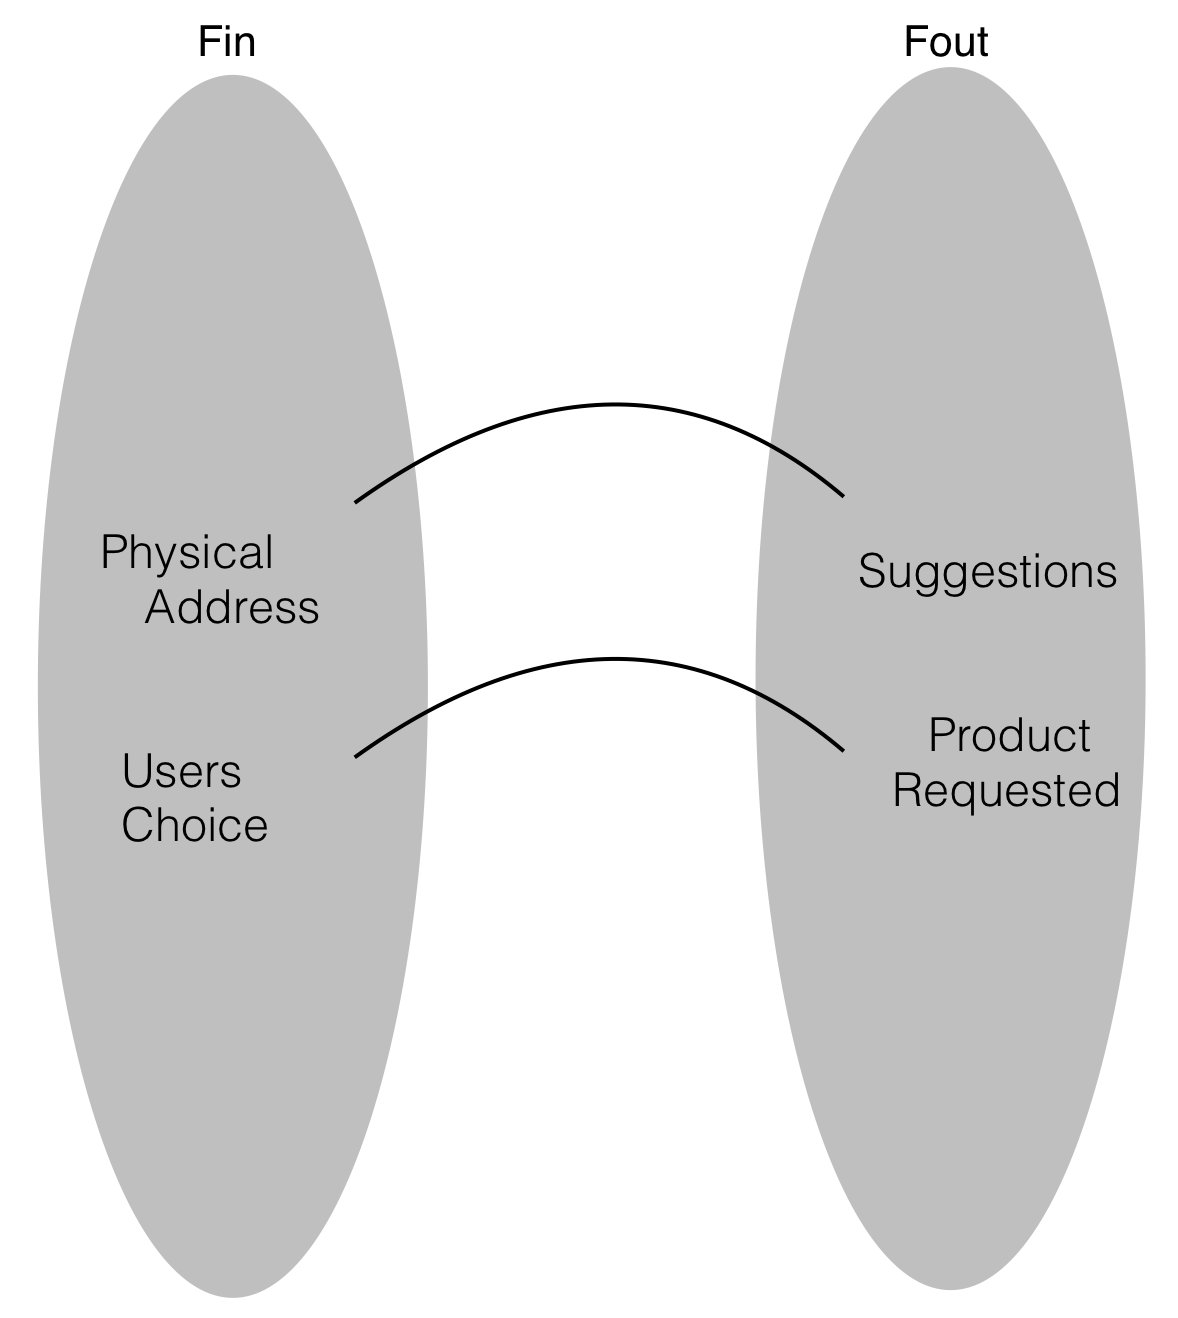
\includegraphics[height=150pt]{function.png}}
	  \caption{Function Diagram}
	  \label{fig:act-dig}
	\end{figure}
\end{center}  
Finitiate :{Fconnectwifi ,Fflashurl,Fconnectaws}\\
Fdetect:{Fdetectwifi}\\
Fconnect:{Fcw ,Fcaws}\\
Fcw :refresh connection wifi\\
Fcaws :refresh connection AWS\\
Ffriend = inbuilt functions.\\
Ffriend = (fproc , fcloud).\\
Non Deterministic Data : Physical address of user's device and location.\\
Deterministic Data :Items(as flashed on users device)\\
Success Conditions:Valid input( i.e valid user choice) is given and the product is dispensed successfully and proper internet availability.\\
Failure Conditions: Invalid input( i.e invalid user choice)  given and product not dispensed along with poor internet availability.\\


\section{Names of Conferences / Journals where papers can be published}

Journal of Internet Services and Applications, January 26-29, 2017. \\
IEEE Cloud Computing,June 25 - June 30, 2017.\\
IEEE International Conference on Communications, 21-25 May 2017.\\
International Journal of Advanced Computing and Technology, 01-​03. ​June 2017\\


\section{Review of Conference/Journal Papers supporting Project idea}
\label{sec:survey}
\begin{enumerate}

\item Zaruba, G.v., S. Basagni, and I. Chlamtac. "Bluetrees-scatternet Formation to Enable Bluetooth-based Ad Hoc Networks." ICC 2001. IEEE International Conference on Communications. Conference Record (Cat. No.01CH37240) (n.d.): n. pag. Web\\
Bluetooth is an open specification for short-range
wireless communication and networking, mainly intended to be
a cable replacement between portable and/or fixed electronic de-
vices. The specification also defines techniques for interconnecting
large number of nodes in scatternets, thus enabling the establish-
ment of a mobile ad hoc network (MANET). While several solutions
and commercial products have been introduced for one-hop Blue-
tooth communication, the problem of scatternet formation has not
yet been dealt with. This problem concerns the assignment of the
roles of master and slave to each node so that the resulting MANET
is connected. In this paper they introduce two novel protocols for
forming connected scatternets. In both cases, the resulting topol-
ogy is termed a bluetree. In our bluetrees the number of roles each
node can assume are limited to two or three (depending on the
protocol), thus imposing low slave management overhead. The ef-
fectiveness of both protocols in forming MANETs is demonstrated
through extensive simulations.\\
\item Linthicum, David S. "The Technical Case for Mixing Cloud Computing and Manufacturing." IEEE Cloud Computing 3.4 (2016): 12-15. Web.\\
Today’s manufacturing processes often lack visibility into resource consumption metrics, productivity, and even logistics. The end result is huge blind spots in the building process that often mean a lack of productivity and efficiency, leading manufacturing companies down unprofitable paths.\\
\item Massuthe, P., and K. Schmidt. "Operating Guidelines - an Automata-Theoretic Foundation for the Service-Oriented Architecture." Fifth International Conference on Quality Software (QSIC'05) (n.d.): n. pag. Web.\\
In the service-oriented architecture (SOA), we distinguish three roles of service owners: service providers, service requesters, and service brokers. Each service provider publishes information to the broker about how requesters can interact with its service. Thus, the broker can assign a fitting service provider to a querying requester. We propose the information published to the broker to be operating guidelines. Operating guidelines are essentially communication instructions for the service requester.
They present an automata-theoretic approach that is centered around operating guidelines and is capable of implementing all tasks arising in the SOA.\\

\item Sneps-Sneppe, Manfred, and Dmitry Namiot. "On Physical Web Models." 2016 International Siberian Conference on Control and Communications (SIBCON) (2016): n. pag. Web.\\
The Physical Web is a generic term describes interconnection of physical objects and web. The Physical Web lets to present physical objects in a web. There are different ways
to do that and we will discuss them in our paper. Usually, the web presentation for a physical object could implement with the help of mobile devices. The basic idea behind the Physical Web is to navigate and control physical objects in the world surrounding
mobile devices with the help of web technologies. Of course, there are different ways to identify and enumerate physical objects. In this paper, they describe the existing models as well as related challenges. In our analysis, we will target objects enumeration
and navigation as well as data retrieving and programming for the Physical Web. \\
\item Namiot, Dmitry, and Manfred Sneps-Sneppe. "The Physical Web in Smart Cities." 2015 Advances in Wireless and Optical Communications (RTUWO) (2015): n. pag. Web.\\
The AWS Cloud Transformation Maturity Model (CTMM) maps the maturity of
an IT organization’s process, people, and technology capabilities as they move
through the four stages of the journey to the AWS Cloud: project, foundation,
migration, and optimization. The objective of the CTMM is to help enterprise IT
organizations understand the significant challenges they might face to adopt
AWS, learn best practices and activities to handle those challenges, and recognize
the signs of maturity or expected outcomes to gauge their maturity and readiness
at every stage. This whitepaper can guide organizations to measure their
readiness for the AWS Cloud, build an effective cloud transformation strategy,
and drive an effective execution plan.\\
\item Lee, Jin-Shyan, Yu-Wei Su, and Chung-Chou Shen. "A Comparative Study of Wireless Protocols: Bluetooth, UWB, ZigBee, and Wi-Fi." IECON 2007 - 33rd Annual Conference of the IEEE Industrial Electronics Society (2007): n. pag. Web.\\
Bluetooth (over IEEE 802.15.1), ultra-wideband(UWB, over IEEE 802.15.3), ZigBee (over IEEE 802.15.4), and Wi-Fi (over IEEE 802.11) are four protocol standards for short-range wireless communications with low power consumption. From an application point of view, Bluetooth is intended for a cordless mouse, keyboard, and hands-free headset, UWB is oriented to high-bandwidth multimedia links, ZigBee is designed for reliable wirelessly networked monitoring and control networks, while Wi-Fi is directed at computer-to-computer connections as an extension or substitution of cabled networks. In this paper, they provide a study of these popular wireless communication standards, evaluating their main features and behaviors in terms of various metrics, including the transmission time, data coding efficiency, complexity, and power consumption.It is believed that the comparison presented in this paper would benefit application engineers in selecting an appropriate protocol.\\
\item Simeone, Osvaldo, and Haim H. Permuter. "Source Coding with Delayed Side Information." 2012 IEEE International Symposium on Information Theory Proceedings (2012): n. pag. Web.\\
We study source coding in the presence of side information, when the system can take actions that affect the availability, quality, or nature of the side information. We begin by extending the Wyner-Ziv problem of source coding with decoder side information to the case where the decoder is allowed to choose actions affecting the side information. We then consider the setting where actions are taken by the encoder, based on its observation of the source. Actions may have costs that are commensurate with the quality of the side information they yield, and an overall per-symbol cost constraint may be imposed. We characterize the achievable tradeoffs between rate, distortion, and cost in some of these problem settings. Among our findings is the fact that even in the absence of a cost constraint, greedily choosing the action associated with the “best” side information is, in general, suboptimal.A few examples are worked out.\\
\item Zhang, Qi, Lu Cheng, and Raouf Boutaba. "Cloud Computing: State-of-the-art and Research Challenges." Journal of Internet Services and Applications 1.1 (2010): 7-18. Web.\\
Cloud computing has recently emerged as a new paradigm for hosting and delivering services over the Internet. Cloud computing is attractive to business owners as it eliminates the requirement for users to plan ahead for provisioning, and allows enterprises to start from the small and increase resources only when there is a rise in service demand. However, despite the fact that cloud computing offers huge opportunities to the IT industry, the development of cloud computing technology is currently at its infancy, with many issues still to be addressed. In this paper, they present a survey of cloud computing, highlighting its key concepts, architectural principles, state-of-the-art implementation as well as research challenges. The aim of this paper is to provide a better understanding of the design challenges of cloud computing and identify important research directions in this increasingly important area.\\
\end{enumerate}   

\section{Plan of Project Execution}

\begin{table}[!htbp]
\begin{center}
%\def\arraystretch{1.5}
\def\arraystretch{1.5}
\begin{tabularx}{\textwidth}{| X | X |}
\hline
Activity	& Planned months\\
\hline
Requirement gathering and feasibility studying        &1 july – 15 Aug\\
\hline
Planning Activities       &16 Aug – 31 Aug\\
\hline
Designing Modules        &1 sept – 31 Oct\\
\hline
Implementation           &1 Nov – 14 Jan\\
\hline
Testing                  &15 Jan – 15 Feb\\
\hline
Deployment               &16 Feb – 28 Feb\\
\hline
\end{tabularx}
\end{center}
\caption{Project Plan}
\label{tab:usecase}
\end{table}
TASK1: Requirement gathering and feasibility studying
\begin{enumerate}
\item Collect Hardware requirements, software requirements. 
\item Study the deployment environment.
\end{enumerate}
TASK2: Planning Activities
\begin{enumerate}
\item Deciding topic with the guide and mentor. 
\item Working on software reqirement gathering.
\end{enumerate}
TASK3: Designing Modules
\begin{enumerate}
\item Create Mockups for web design. 
\item Create use case and other charts for clear functional understanding.
\end{enumerate}
TASK4: Implementation
\begin{enumerate}
\item Start with the Web development.
\item Database interfacing.
\end{enumerate}
TASK5: Testing 
\begin{enumerate}
\item Testing the vendor side application flow.
\item Testing the user side application.
\end{enumerate}
TASK6: Deployment
\begin{enumerate}
\item Deploy the application.
\item Proper documentation is also provided.
\end{enumerate}
\subsubsection{TimeLine Chart}
\begin{center}
	\begin{figure}[!htbp]
		\centering
		\fbox{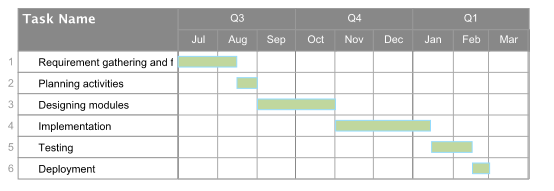
\includegraphics[height=150pt]{gantt.png}}
	  \caption{Timeline Chart}
	  \label{fig:act-dig}
	\end{figure}
\end{center}  
\newpage


\chapter{Technical Keywords}
\section{Area of Project}
Internet of Things
\section{Technical Keywords}
% {\bfseries Technical Key Words:}      
% \begin{itemize}
%   \item 	Cloud Computing
% \item	Service Composition
% \item	Online Web services
% \end{itemize}

$\bullet$ Computer systems organization\\ 
Distributed architecure\\
- Cloud computing \\
- Client server architectures\\
$\bullet$ Embedded and cyber-physical systems\\
Embedded systems\\
-Embedded hardware\\
 
\chapter{Introduction}
\section{Project Idea}

 We are proposing a platform for vending machine functionalities and management to be  handled by cloud using Internet of things.Online payment for vending machines made possible and stock record maintained on the cloud for dynamically updating the vendor .


\section{Motivation of the Project}  

 Presently the people use coins or paper money while operating the vending machines due to this there arises a problem when the user does not seem to have exact change with him and the vendors dont come to know about the stock required in the vending machines when excess usage is done.Hence to minimize these problems we provide an efficient solution.

\section{Literature Survey}
 Physical Web with Vending machine.\\
Papers referred: Refer to Paper Reveiw part given before.\\
Background content:\\
AWS Services: Amazon Web Services offers reliable, scalable, and inexpensive cloud computing services.\\
AWS IoT: It is a platform that enables you to connect devices to AWS Services and other devices, secure data and interactions, process and act upon device data, and enable applications to interact with devices even when they are offline.\\
Amazon EC2: Amazon Elastic Compute Cloud is a web service that provides resizable compute capacity in the cloud. It is designed to make web-scale cloud computing easier for developers.\\
Amazon S3: Amazon Simple Storage Service is storage for the Internet. It is designed to make web-scale computing easier for developers.\\
Amazon RDS: Amazon Relational Database Service (Amazon RDS) is a web service that makes it easier to set up, operate, and scale a relational database in the cloud. It provides cost-efficient, resizeable capacity for an industry-standard relational database and manages common database administration tasks. \\
Beacons:  Give users a better location and proximity experiences by providing a strong context signal for their devices in the form of Bluetooth low energy (BLE) beacons with Eddystone, the open beacon format from Google. \\
Eddystone: It is an open beacon format from Google that works with Android and iOS. The process of setting up a beacon to broadcast (sometimes called 'provisioning') can be completed using Google's Beacon Tools app for Android and iOS, using a tool from your manufacturer, or sometimes in bulk by prior arrangement with the beacon manufacturer. \\
Beacons can be deployed at fixed places such as airports, museums, and bus stops, and attached to movable objects such as bicycles, kiosks, and taxis.\\


\begin{table}[!htbp]
\begin{center}
%\def\arraystretch{1.5}
\def\arraystretch{1.5}
\begin{tabularx}{\textwidth}{| X | X | X | X | X |}
\hline
Parameters	&Paper1 &Paper2 &Paper3 &Paper4\\
\hline
Topic       &Cloud computing: State -of-the-Art and Research challenges &On Physical Web Models. &Bluetrees-scatternet Formation to Enable Bluetooth-based Ad Hoc Networks. &A Comparative Study of Wireless Protocols: Bluetooth, UWB, ZigBee, and Wi-Fi.\\
\hline

Paper Type      &Journal &Research  &Study  &Conference\\
\hline

Objective      & To present a survey of cloud computing, highlighting its key concepts, architectural principles, state-of-the-art implementation as well as research challenges.& The existing physical web models as well as related challenges are described in this paper. &Two novel protocols for forming connected scatternets are introduced. &To provide a study of these popular wireless communication standards.\\
\hline

Result &To provide a better understanding of the design challenges of cloud computing and identify important research directions in this increasingly important area. &Objects enumeration and navigation as well as data retrieving and programming for the Physical Web. &The effectiveness of both protocols in forming MANETs is demonstrated
through extensive simulations. &Study of these popular wireless communication standards, evaluating their main features and behaviors in terms of various metrics, including the transmission time, data coding efficiency, complexity, and power consumption made.\\
\hline


\end{tabularx}
\end{center}
\caption{Literature Survey}
\label{tab:usecase}
\end{table}



\chapter{Problem Definition and scope}
\section{Problem Statement}
 To automate vending machine functionalities for vendors and enabling easy accessibility for users through online payment and establishing a physical interface with the help of beacons. 


\subsection{Goals and objectives}  
Project Goal:
\begin{enumerate}
\item Interactive vending machine with cashless payment and cloud
connectivity.
\item Enhanced User experience by using visualization for dynamic data
change through web applications.
\end{enumerate}	
Project Objectives:
\begin{enumerate}
\item User authentication and a simple signup/signin form.
\item To create a URL redirection and a simple CMS for the webpages. 
\item Database creation and connectivity.
\item Developing  Vendor page and user page.
\item Add Payment functionality uing Paytm API.
\item Study the parameters for Vending Machine.
\item Connectivity between vending machine and cloud.
\item Testing the Application. 
\end{enumerate}	

 \subsection{Statement of scope} 
This project will consist of creating a platform for vending machine functionalities and management to be  handled by cloud using Internet of things.Online payment for vending machines is made possible and stock record is maintained on the cloud for dynamically updating the vendor. Modules of the platform will include a firmware where hardware is used,cloud communication and a frontend available for users as well as for vendors respectively.\\
Type of vending machine : Product base.
Products: Bisleri,  coca cola and other beverages.
Device type : Mobiles which support chrome browser (e.g.Android/ios)\\
Limit of the project will be internet dependency ,so better connection (3Mbps) is required.\\
Functionality mechanism is concentrated on removing the cash payment barrier on the vending machine .\\
Final product will be used at public places like railway stations,airports,bus stands and can be used by private vendors.\\
\section{Software context}
The project will be effectively used at public places where vending machine's are placed.\\
Places like Airports, Railway stations, Bus stands and other public places have this facility coming up to support the Digital India initiative by going cashless.\\

\section{Major Constraints}
Need of google chrome browser: The user should have google chrome browser to take advantage of this service as currently the web bluetooth technology is supported by only google chrome. \\
Availability of Wi-Fi connections: The vending machine should be placed in the place where wifi availability is there ,for smoother connection and faster product delivery.If the internet fluctuates then user will have to wait for product and this in turn lead to decrease in product sale.\\
Location of the vending machines: Vending machine should be placed where it can be accesible to the people i.e the bluetooth range.\\

\section{Scenario in which multi-core, Embedded and Distributed Computing used}

We will have a Wi-Fi enabled board on the vending machines which will send beacons to the mobile phones having Bluetooth in their vicinity.\\
The user will receive a notification which will contain a URL flashed by the beacon on his cellphone along with suggestions for other products.\\
The user will hence find and approach the vending machine and click on the desired product on his cellphone.\\
The transaction is carried out using the online payment gateways or mobile wallet and is recorded and stored in the cloud which is used for future transactions.\\
The vending machine then dispenses the product ordered by the user.\\
The vendor will have an updated list of the stock remaining in the cloud.

\section{Outcome}

 Online (cashless) payments are available for the users for easy purchase of items.
Vendors are well informed about the stock management of the machine and they are also aware of the customers past transactions.

\section{Applications}

Vending machines in airports,malls and offices.

\section{Hardware Resources Required}
\begin{enumerate}
\item Beacons (Eddystone Bluetooth 4.0 protocol).
\item Vending machines.
\item Knit board(wifi-enabled micro controller).
\item Mobile phone.(Android(Version: 6.0) or iOS(version: 8))
\end{enumerate}


\section{Software Resources Required}
Platform : Amazon Web Services.
\begin{enumerate}
\item Operating System:Linux(Ubuntu16.04). 
\item IDE: Eclipse (Mars).(3.0)
\item Programming Language : C , javascript
\item API: Web Bluetooth(4.0)
\item AWSIOT Device SDK JS (Version 1.0.12)
\item Google chrome Browser (version :53.0.2785.143)
\end{enumerate}




\chapter{Project Plan}

\section{Project Estimates}
 Our project is based on an Incremental Model. 
 
\subsubsection{Time Estimates}

\begin{table}[!htbp]
\begin{center}
%\def\arraystretch{1.5}
\def\arraystretch{1.5}
\begin{tabularx}{\textwidth}{| X | X |}
\hline
Activity	& Planned months\\
\hline
Requirement gathering and feasibility studying        &1 july – 15 Aug\\
\hline
Planning Activities       &16 Aug – 31 Aug\\
\hline
Designing Modules        &1 sept – 31 Oct\\
\hline
Implementation           &1 Nov – 14 Jan\\
\hline
Testing                  &15 Jan – 15 Feb\\
\hline
Deployment               &16 Feb – 28 Feb\\
\hline



\end{tabularx}
\end{center}
\caption{Project Plan}
\label{tab:usecase}
\end{table}
\newpage
\subsection{Project Resources}
\begin{enumerate}
\item Beacons.
\item Vending machines.
\item Knit board(wifi-enabled micro controller).
\item Mobile phone.(Android(Version: 6.0) or iOS(version: 8))
\item Operating System:Linux(Ubuntu16.04). 
\item IDE: Eclipse (Mars).(3.0)
\item Programming Language : C , javascript
\item API: Web Bluetooth(4.0)
\item AWSIOT Device SDK JS (Version 1.0.12)
\item Google chrome Browser (version :53.0.2785.143)
\end{enumerate}
\section{Risk Management w.r.t. NP Hard analysis}
Project Risks \\
The dependency on google chrome browser: The user should have google chrome browser to take advantage of this service as currently the web bluetooth technology is supported by only google chrome.\\
Fluctuations of Wi-Fi connections: The vending machine should be placed in the place where wifi availability is there ,for smoother connection and faster product delivery.If the internet fluctuates then user will have to wait for product and this in turn lead to decrease in product sale.\\
Location of the vending machines: Vending machine should be placed where it can be accesible to the people i.e the bluetooth range.\\
 
\subsection{Risk Identification}
\begin{enumerate}
\item Have top software and customer managers formally committed to support the project?\\
Yes,the top software company manager has approved our idea and is fully committed to support our project.
\item Are end-users enthusiastically committed to the project and the system/product to be built?\\
The end users in our case being the vendors are happy about the change and betterment we will bring in their bussiness with our platform.
\item Are requirements fully understood by the software engineering team and its customers?\\
The requirements are understood completely and are taken care of by the software engineering team and its customers.
\item Have customers been involved fully in the definition of requirements?\\
The customera are involved and are supporting us for the development of the platform.
\item Do end-users have realistic expectations?\\
 Yes the users do have realistic expectations as our platform will bring a betterment and improve their means of bussiness.
\item Does the software engineering team have the right mix of skills?\\
The software engineering team is the finest we can meet and are at par with their skills.
\item Are project requirements stable?\\
 The project requirements are stable and simple.
\item Is the number of people on the project team adequate to do the job?\\
Yes the number of people on this project are adequate.
\item Do all customer/user constituencies agree on the importance of the project and on the requirements for the system/product to be built?\\
 The customers agree with our idea and are eager to support us in our endeavour.
\end{enumerate}

\subsection{Risk Analysis}
The risks for the Project can be analyzed within the constraints of time and quality

\begin{table}[!htbp]
\begin{center}
%\def\arraystretch{1.5}
\def\arraystretch{1.5}
\begin{tabularx}{\textwidth}{| c | X | c | c | c | c |}
\hline
\multirow{2}{*}{ID} & \multirow{2}{*}{Risk Description}	& \multirow{2}{*}{Probability} & \multicolumn{3}{|c|}{Impact} \\ \cline{4-6}
	& & &	Schedule	& Quality	& Overall \\ \hline
1	& Location of vending machine	& Low	& Low	& High	& High \\ \hline
2	& Availability of WiFi connections	& Low	& Low	& High	& High \\ \hline
\end{tabularx}
\end{center}
\caption{Risk Table}
\label{tab:risk}
\end{table}


\begin{table}[!htbp]
\begin{center}
%\def\arraystretch{1.5}
\def\arraystretch{1.5}
\begin{tabular}{| c | c | c |}
\hline
Probability & Value &	Description \\ \hline
High &	Probability of occurrence is &  $ > 75 \% $ \\ \hline
Medium &	Probability of occurrence is  & $26-75 \% $ \\ \hline
Low	& Probability of occurrence is & $ < 25 \% $ \\ \hline
\end{tabular}
\end{center}
\caption{Risk Probability definitions \cite{bookPressman}}
\label{tab:riskdef}
\end{table}

\begin{table}[!htbp]
\begin{center}
%\def\arraystretch{1.5}
\def\arraystretch{1.5}
\begin{tabularx}{\textwidth}{| c | c | X |}
\hline
Impact & Value	& Description \\ \hline
Very high &	$> 10 \%$ & Schedule impact or Unacceptable quality \\ \hline
High &	$5-10 \%$ & Schedule impact or Some parts of the project have low quality \\ \hline
Medium	& $ < 5 \% $ & Schedule impact or Barely noticeable degradation in quality Low	Impact on schedule or Quality can be incorporated \\ \hline
\end{tabularx}
\end{center}
\caption{Risk Impact definitions \cite{bookPressman}}
\label{tab:riskImpactDef}
\end{table}

\subsection{Overview of Risk Mitigation, Monitoring, Management}


Following are the details for each risk.
\begin{table}[!htbp]
\begin{center}
%\def\arraystretch{1.5}
\def\arraystretch{1.5}
\begin{tabularx}{\textwidth}{| l | X |}
\hline 
Risk ID	& 1 \\ \hline
Risk Description	& Location of the vending machine.\\ \hline
Category	& Development Environment. \\ \hline
Source	& Software requirement Specification document. \\ \hline
Probability	& Low \\ \hline
Impact	& High \\ \hline
Strategy &Do the environment study and then place bluetooth devicefor respective machine \\ \hline
Risk Status	& Identified \\ \hline
\end{tabularx}
\end{center}
%\caption{Risk Impact definitions \cite{bookPressman}}
\label{tab:risk1}
\end{table}

\begin{table}[!htbp]
\begin{center}
%\def\arraystretch{1.5}
\def\arraystretch{1.5}
\begin{tabularx}{\textwidth}{| l | X |}
\hline 
Risk ID	& 2 \\ \hline
Risk Description	& Availability of the WiFi connection.\\ \hline
Category	& Requirements \\ \hline
Source	& Software Design Specification documentation review. \\ \hline
Probability	& Low \\ \hline
Impact	& High \\ \hline
Strategy	& Better testing will resolve this issue.  \\ \hline
Risk Status	& Identified \\ \hline
\end{tabularx}
\end{center}
\label{tab:risk2}
\end{table}
\newpage
\section{Project Schedule}  
\subsection{Project task set}  
Major Tasks in the Project stages are:\\
Task 1: Requirement gathering and feasibility studying.\\
Task 2: Planning Activities.\\
Task 3: Designing Modules\\
Task 4: Implementation. \\
Task 5: Testing.\\
Task 6: Deployment.\\

\subsection{Task network}  
Project tasks and their dependencies are noted in this diagrammatic form.
\begin{center}
	\begin{figure}[!htbp]
		\centering
		\fbox{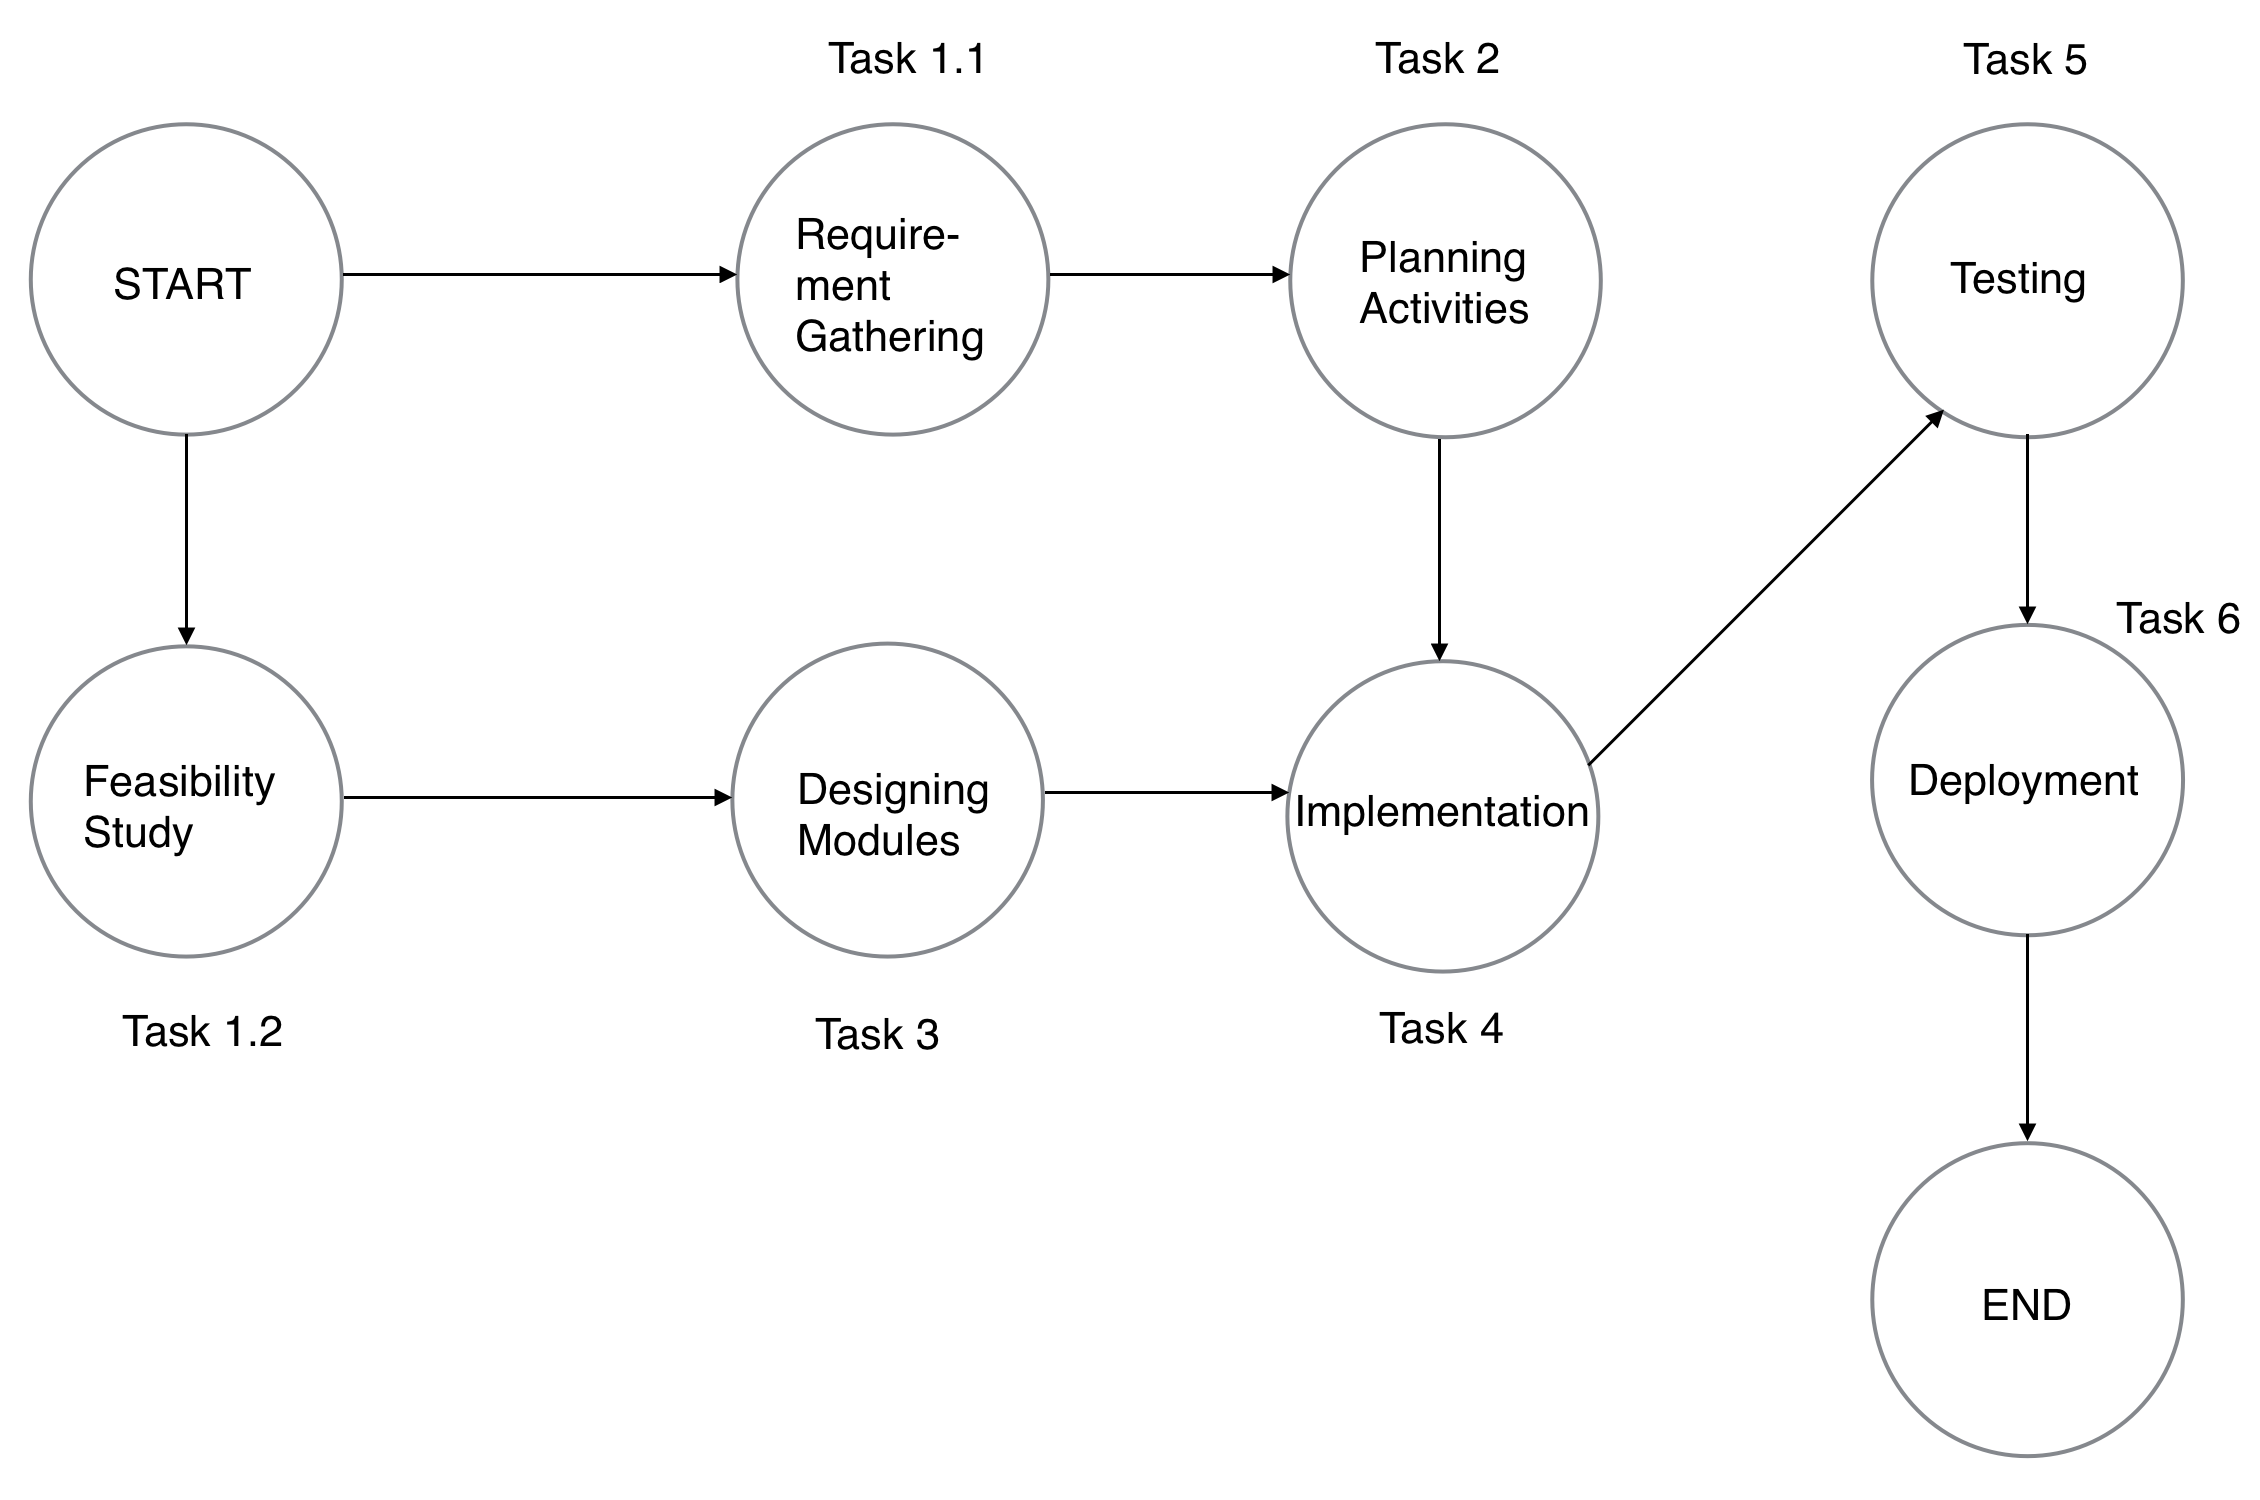
\includegraphics[height=250pt]{tn.png}}
	  \caption{Task Network}
	  \label{fig:act-dig}
	\end{figure}
\end{center}  
This diagram describes the flow of various tasks.In the figure the tasks are performed in the following manner:\\
Task 1-The hardware is initiated initially.\\
Task 2- Wifi connection established.\\
Task 3- Activate the beacons.\\
Task 4-Establish cloud communication.\\
Task 5-Flash the URL on the user's phone.\\
Task 6-The user finds the vending machine and product is purchased.\\
Finally the inventory of the vendor is updated.\\
\newpage

\subsection{Timeline Chart}  

\begin{center}
	\begin{figure}[!htbp]
		\centering
		\fbox{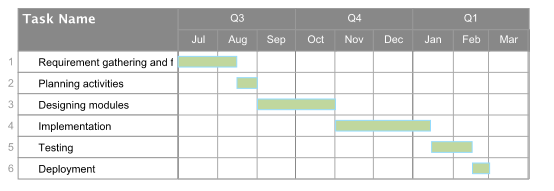
\includegraphics[height=150pt]{gantt.png}}
	  \caption{Timeline Chart}
	  \label{fig:act-dig}
	\end{figure}
\end{center}  



 
\section{Team Organization}
\subsection{Team structure}
College Guide - Prof A.R.Deshpande\\
Mentor - Mr. Anuj Deshpande \\
Group members -\\
Sejal Khatri\\
Amruta Ranade\\
Kevin Kaul\\
Our project is divided into different smaller modules and the team works independently on  different modules.


\subsection{Management reporting and communication}
We communicate with our college guide and mentor on a regular basis.A log record is maintained which consists of the progress records.
Meetings are conducted with our mentor once every week and the development is recorded.
\chapter{Software reqirement specification  (SRS is to be prepared using relevant mathematics derived and software engg. Indicators in Annex A and B)}

\section{Introduction}
\subsection{Purpose and Scope of Document}
Purpose:\\
This SRS is written in precise, clear and plain language.In depth analysis of all the vending machine's hardware and software requirements is performed.
The analytical models (use case diagrams, entity relationship diagrams, data flow diagram etc.) are used for the detailed design and the development of the software system. SRS is one of
the most critical pieces of software development since it acts as the bridge betweens the
software developers and business analysts.\\
Scope:\\
Primarily, the scope pertains to the Vending machine providing services to the user and the
vendor. It focuses on the vendor, which allows for the sales, distribution and marketing of the
products through the vending machine.
This SRS is also aimed at specifying requirements of product to be developed but it can also be
applied to assist in the selection of in-house and commercial software products. The standard can
be used to create software requirements specifications directly or can be used as a model for
defining a organization or project specific stan\\
\subsection{Overview of responsibilities of Developer}
The developer will carry out the following activities:
\begin{enumerate}

\item Requirement gathering
\item Planning of the project
\item Designing various modules
\item Implementation of the project
\item Testing of the modules (white box and black box)
\item Deployment of the product (real life usage)

\end{enumerate}

\section{Usage Scenario}
\subsection{User profiles}  
There are two actors involved in the use case diagram.\\
1. User\\
2. Vendor\\
The user is the person who approaches the vending machine to buy a product and the vendor is the person who sells various products by regularly stocking them up in the vending machine. The relationship between them is similar to a buyer and seller.\\
Use Case 1: User connects to AWS cloud.\\
Use Case 2:Vendor connects to AWS cloud.
Use Case 3:User interacts with the vending machine through cloud.\\

\subsection{Use Case View}
Use Case Diagram. Example is given below
\begin{center}
	\begin{figure}[!htbp]
		\centering
		\fbox{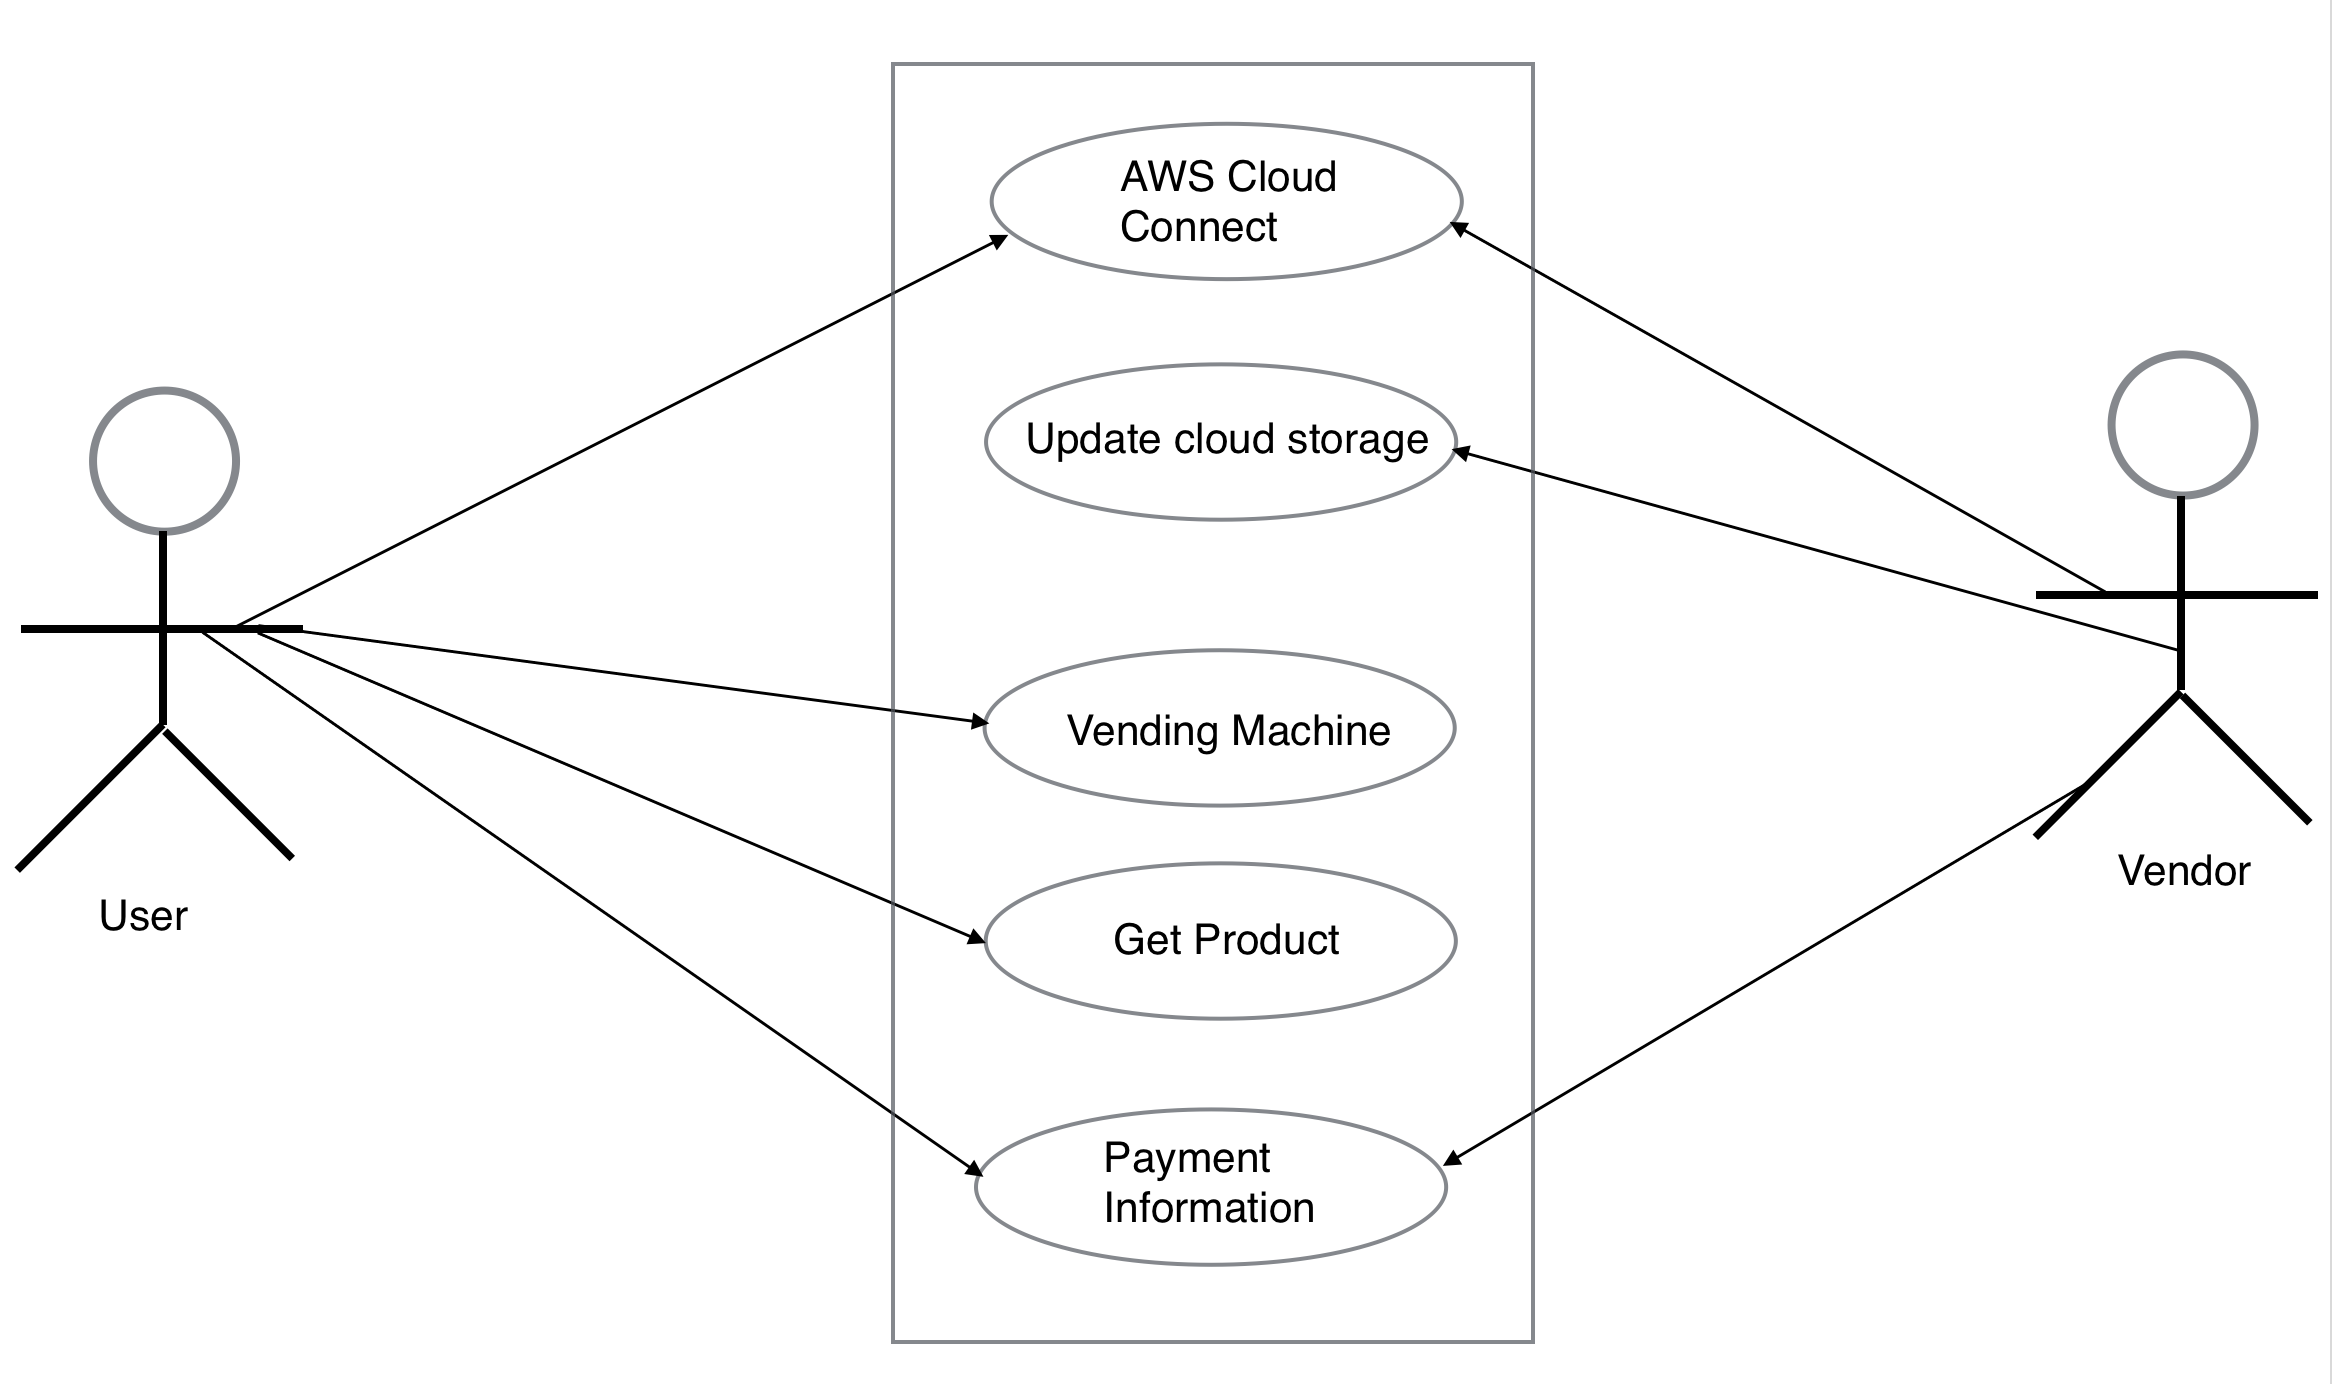
\includegraphics[width=\textwidth]{uc.png}}
	  \caption{Use case diagram}
	  \label{fig:usecase}
	\end{figure}
\end{center}  
\newpage
Description:
The project is consisting of two actors. They are, the user and the vendor. There are five functions, namely, AWS cloud connection, updating cloud storage, using the vending machine, getting the product and payment information.\\
The user and the vendor both interact by using the cloud connection. Both of them also have access to the payment information. The user also uses the vending machine to get the product. On the other hand the vendor is able to update the cloud storage.\\
\section{Data Model and Description}  
\subsection{Data objects and Relationships}
  \begin{center}
	\begin{figure}[!htbp]
		\centering
		\fbox{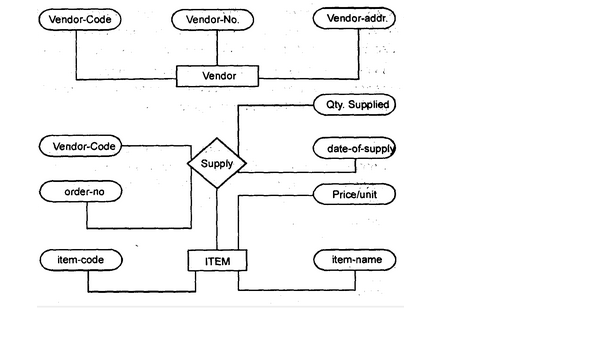
\includegraphics[width=\textwidth]{erd.png}}
	  \caption{ERD diagram}
	  \label{fig:usecase}
	\end{figure}
\end{center}  
\newpage
This diagram depicts the relationship between different entities. We have shown the relationship and functioning taking place between the user and the vendor respectively.\\


\section{Functional Model and Description}  
Our project consists of these software functions--\\
Interfacing knit board with the vending machine.
In this function we are writing codes and storing them on the stlink programmer.
The stlink works with both its end, one end is connected to the vending machine's motors and the other end is connected to the knit board.
Using the flash process we will store and use the code dynamically.\\

Knit board to AWS (Amazon Web Services)--\\
In this function we will connect the knit board functionalities to the cloud server.
This will be done via the REST(Representational state transfer) protocol.\\

REST : They are one way of providing interoperability between computer systems on the internet. REST-compliant web services allow requesting systems to access and manipulate textual representations of web resources using a uniform and predefined set of stateless operations.  \\
There are six guiding constraints that define a RESTful system.These constraints restrict the ways that the server may process and respond to client requests so that, by operating within these constraints, the service gains desirable non-functional properties, such as performance, scalability, simplicity, modifiability, visibility, portability, and reliability.If a service violates any of the required constraints, it cannot be considered RESTful.\\

Cloud to Device(vendor's side)--\\
In this function we will connect the cloud to the Vendor's device through a mqtt protocol.
Mqtt(MQ Telemetry Transport ) Protocol :\\
It is an ISO standard (ISO/IEC PRF 20922)publish-subscribe-based "lightweight" messaging protocol for use on top of the TCP/IP protocol. It is designed for connections with remote locations where a "small code footprint" is required or the network bandwidth is limited.
Further the vendor will have his own database server where all the data collected will be stored and saved.Here various algorithms will be applied to find the location of the vending machine which needs the reloading of products.
We are providing a platform to the vendors such that they will be able to store the user's past transaction history as well.\\


\begin{center}
	\begin{figure}[!htbp]
		\centering
		\fbox{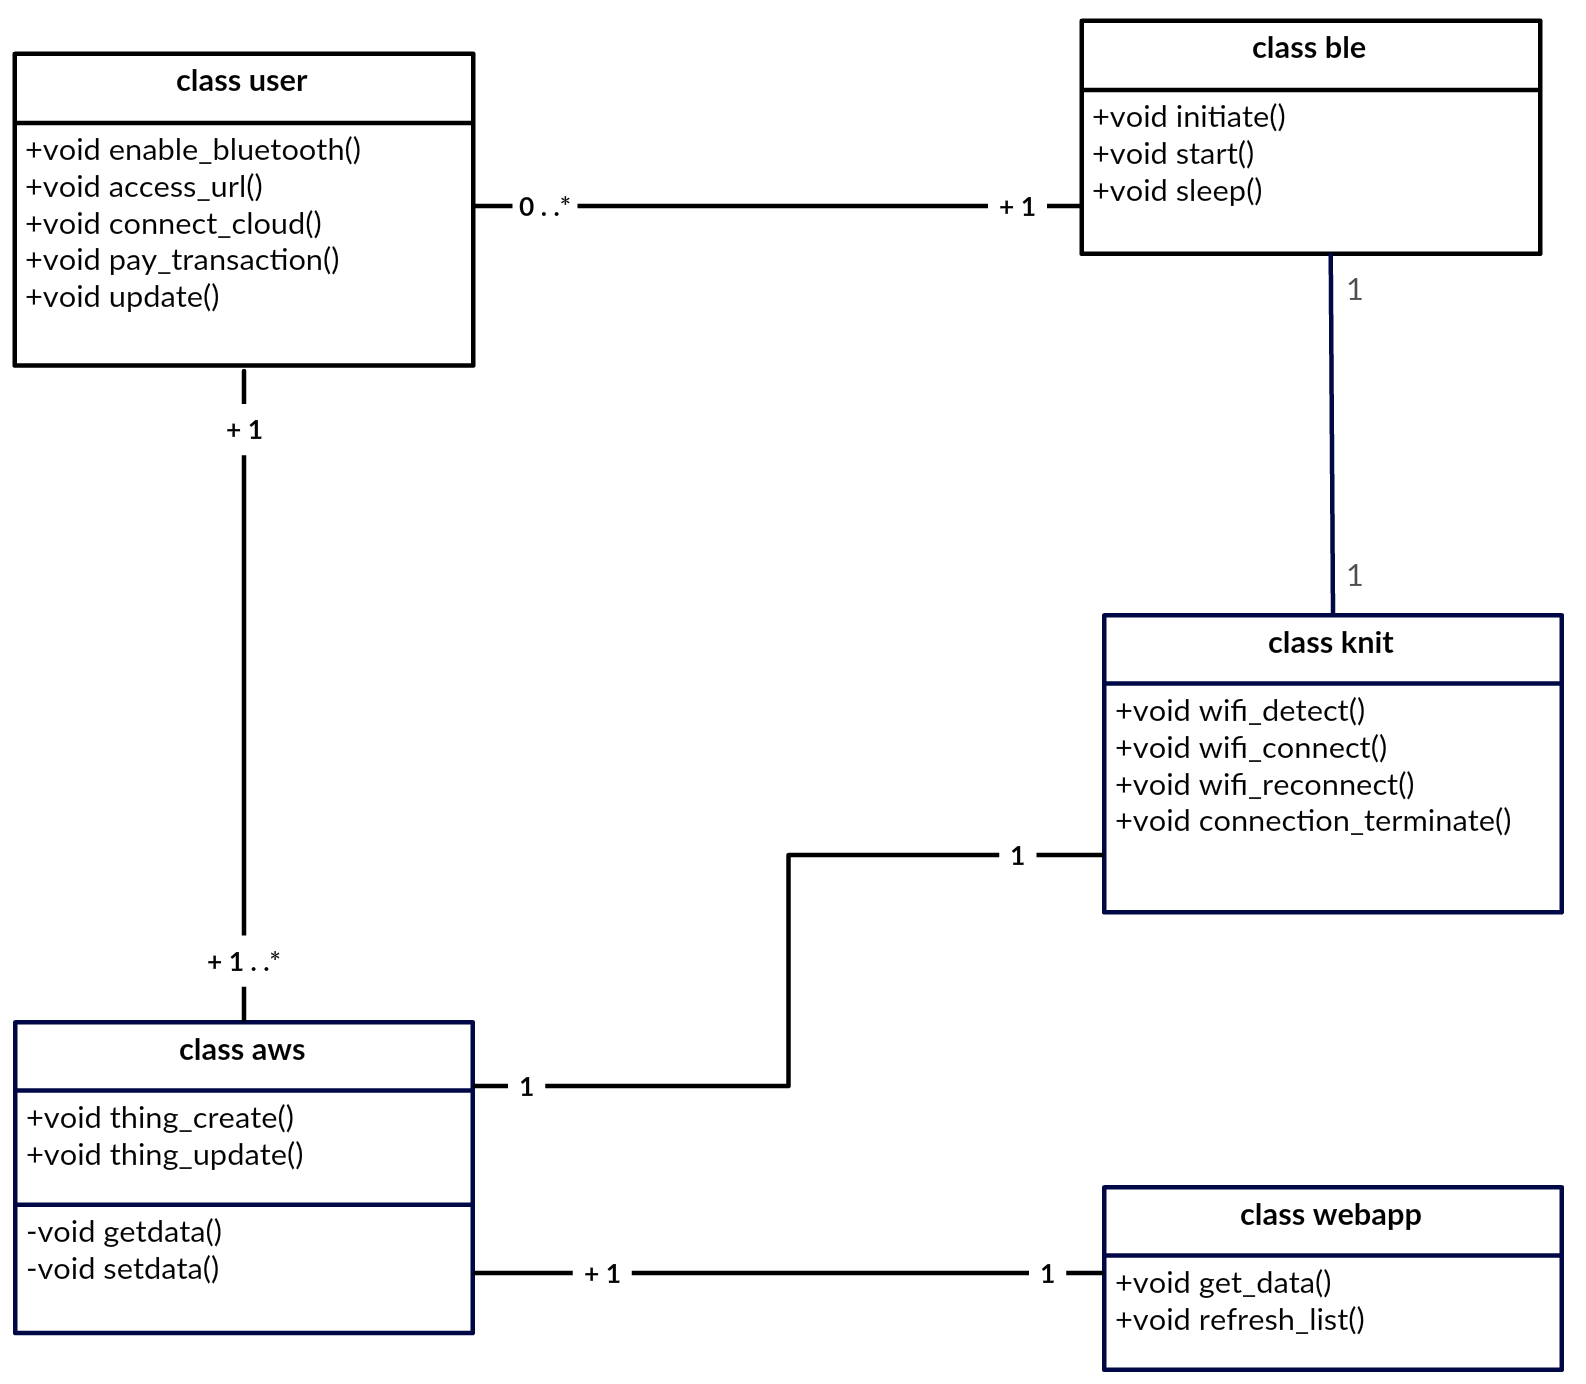
\includegraphics[height=330pt]{class.png}}
	  \caption{Class diagram}
	  \label{fig:act-dig}
	\end{figure}
\end{center}  
\newpage 
This diagram depicts the various classes present in the program and the respective data types and functions used in them.\\
\subsection{Description of functions}  

Fme = Main functions.\\
Fme = (fin , fout,initiate,detect,connect).\\
Fin : {Faddress , Fchioce}\\
Faddress is the function to get user device address and store it in the database .
Fchoice is the function which maps users choice with his particular id ,which further can be used for data analysis \\
Fout:{Fdispose , Fsuggest}\\
Fdispose is the function which is used to validate if payment is done or not and accordingly dispose the product from the vending machine.\\
Fsuggest is the function which suggests product to the user after anlysing its previous choice of products .\\
Finitiate :{Fconnectwifi ,Fflashurl,Fconnectaws}\\
Fconnectwifi :function to connect to the wifi once the device is initiated\\
Fflashurl This function is used to wake up beacon and make it flash url\\
Fconnectaws is used to connect knit board to AWS once its connected to the wifi\\
Fdetect:{Fdetectwifi}\\
Fconnect:{Fcw ,Fcaws}\\
Fcw :refresh connection wifi\\
Fcaws :refresh connection AWS\\
\subsection{Activity Diagram:}

\begin{center}
	\begin{figure}[!htbp]
		\centering
		\fbox{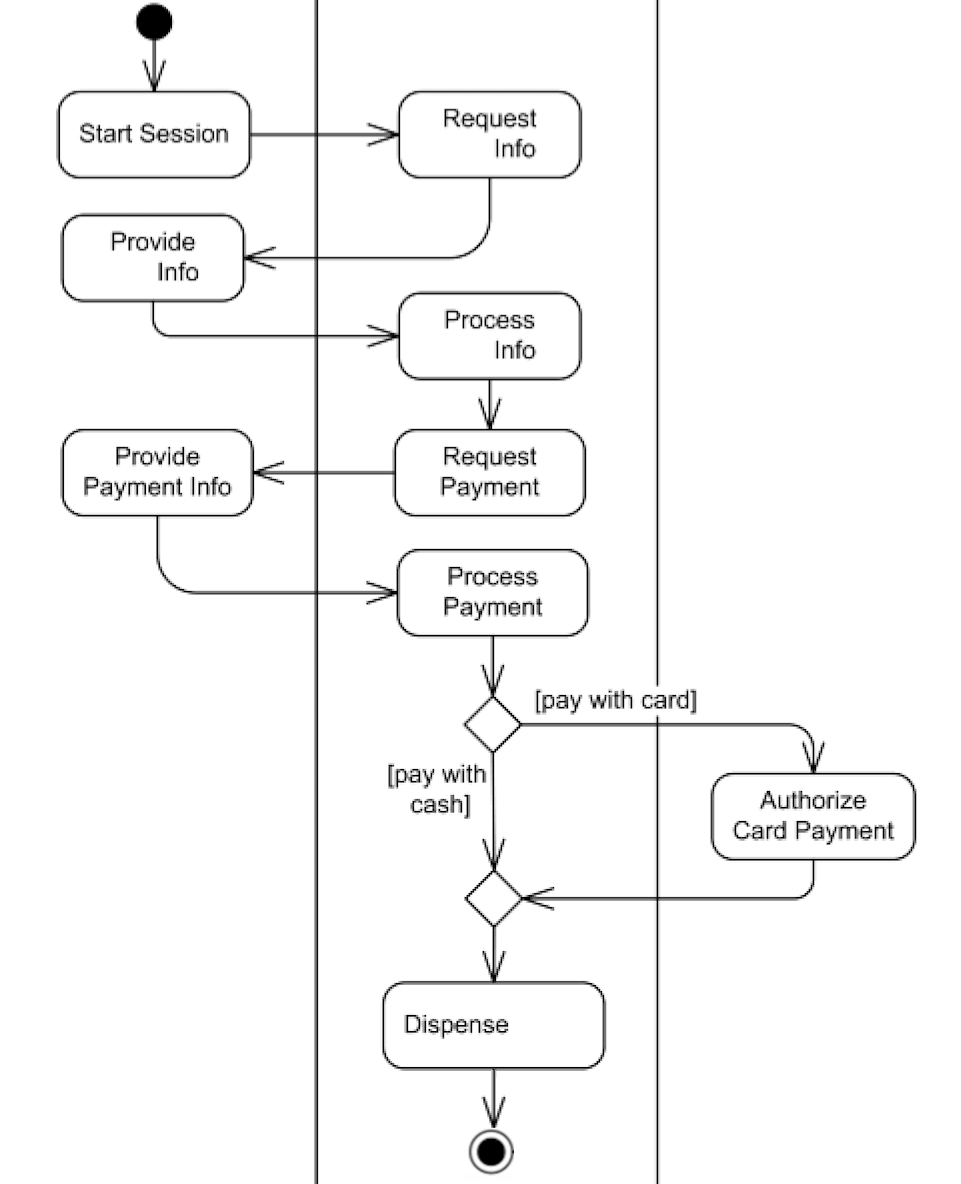
\includegraphics[height=430pt]{ad.png}}
	  \caption{Activity diagram}
	  \label{fig:act-dig}
	\end{figure}
\end{center}  

\newpage


\subsection{State Diagram:}	
  State Transition Diagram\\

\begin{center}
	\begin{figure}[!htbp]
		\centering
		\fbox{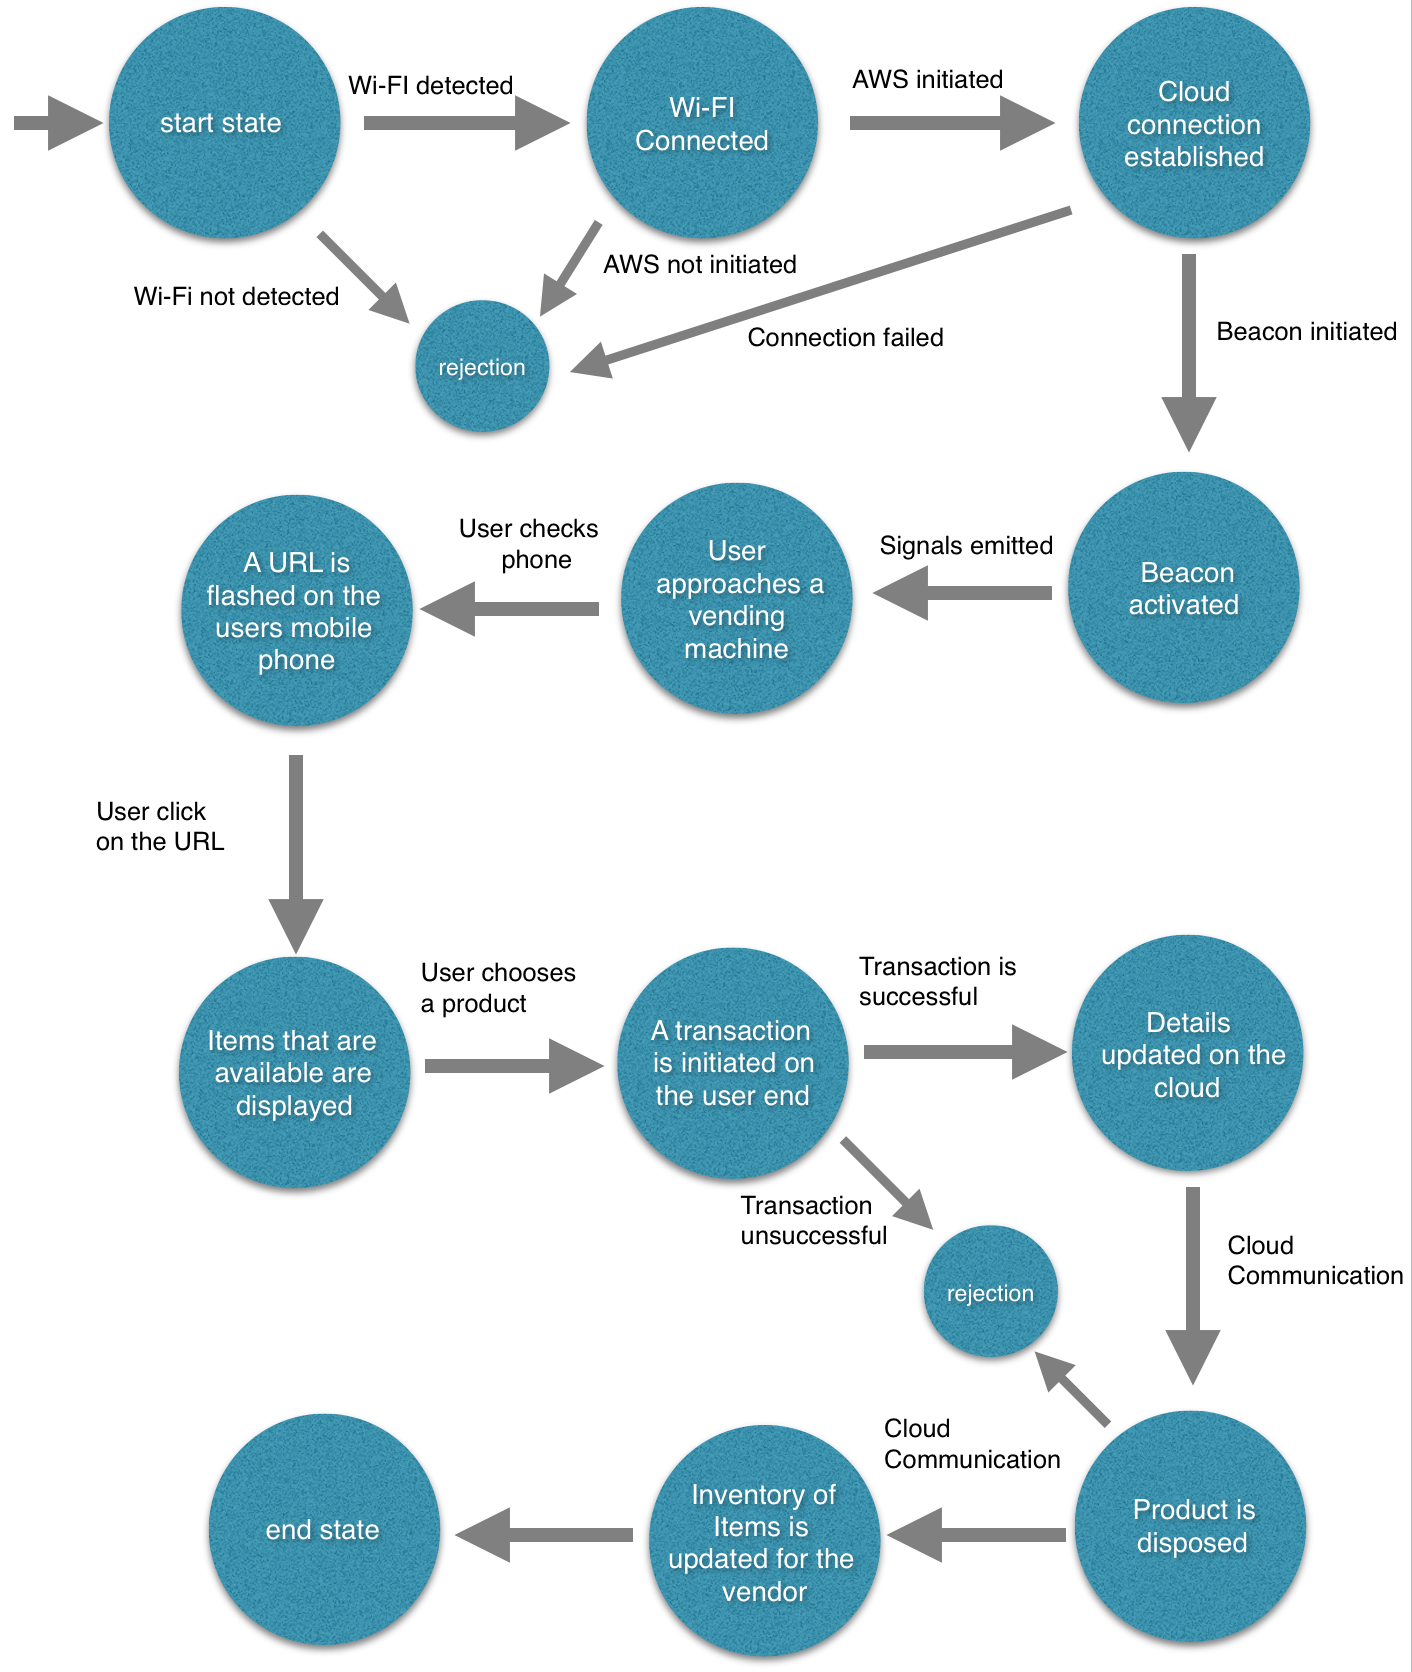
\includegraphics[width=450pt]{state.png}}
	  \caption{State transition diagram}
	  \label{fig:state-dig}
	\end{figure}
\end{center} 
\newpage
This diagram describes the behaviour of the system.\\
State1: Initially is the start state,where the availability of wifi connection is checked.\\
State2: If wifi is detected then system displays the message Wifi connected and if not then the system rejects the user.\\
State3: Next it checks whether the AWS is initiated or not.Once it is, then the cloud communication is established.\\
State4: Once this communication is established,the beacons are activated and the signals are emmitted from them to the user's phone.\\
State5: The user then approaches the vending machine and simultaneously a URL is flashed on the user's mobile phone.\\
State6: Once the user clicks on the URL available items are displayed on his phone.\\
When the user chooses a product ,a transaction is initiated on the user end.\\
State7: If the transaction is successful,the details are updated on the cloud otherwise are rejected.\\
State8: After updation the product is dispensed from the vending machine.and the inventory of items is updated at the vendor side.\\
Hence the process states end.

\subsection{Software Interface Description}	 
Hardware Interface: \\
Hardware interfacing is done at the vending machine side, the driver interfacing for product delivery.\\
Software Interface:\\
Software interfacing is done between knit board (wifi enabled board) and Amazon web services  using aws iot js sdk .So the data is updated in time intervals to the cloud .Concept called thing shadows is used at the cloud side to dynamically update data .\\
Human Interface:\\
Interfacing is also done between cloud and vendor device for dynamically informing the vendor about changed/updated data at the AWS .\\
Payment platform interfacing is done at the user side and with the cloud for proper transaction.\\
\chapter{Detailed Design Document using Appendix A and B}
 \section{Introduction}  
We will have a Wi-Fi enabled board on the vending machines which will send beacons to the mobile phones having Bluetooth in their vicinity.\\
The user will receive a notification which will contain a URL flashed by the beacon on his cellphone along with suggestions for other products.\\
The user will hence find and approach the vending machine and click on the desired product on his cellphone.\\
The transaction is carried out using the online payment gateways or mobile wallet and is recorded and stored in the cloud which is used for future transactions.\\
The vending machine then dispenses the product ordered by the user.\\
The vendor will have an updated list of the stock remaining in the cloud.\\
\section{Architectural Design}  
  \begin{center}
	\begin{figure}[!htbp]
		\centering
		\fbox{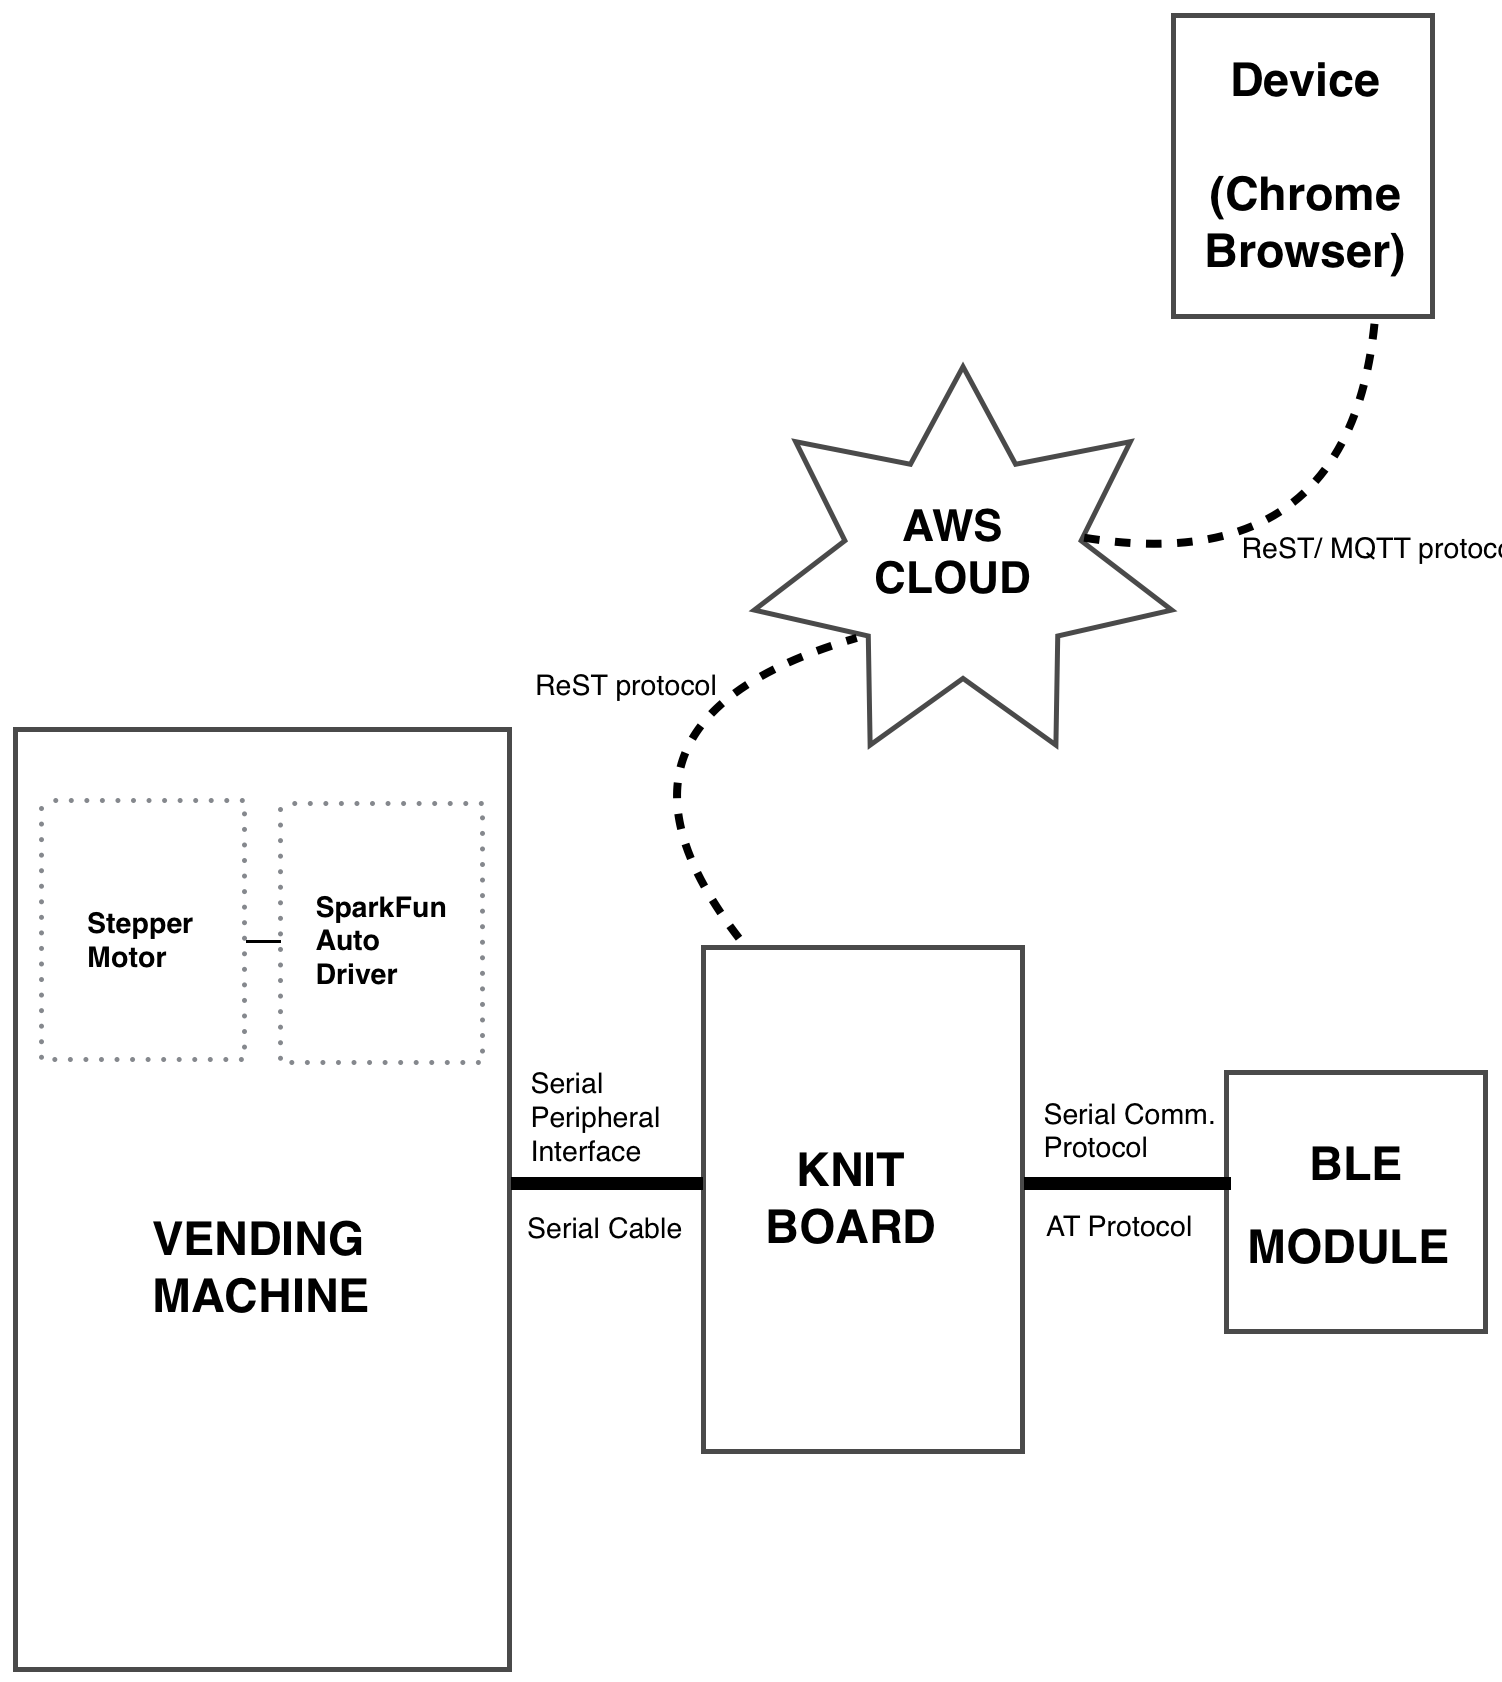
\includegraphics[width=\textwidth]{Arch.png}}
	  \caption{Architecture diagram}
	  \label{fig:arch-dig}
	\end{figure}
\end{center} 
\newpage
In this diagram the knit board is interfaced with the vending machine through a serial peripheral cable.The vending machine consists of stepper motor and drivers used in the process of interfacing with the knit board.A Bluetooth Low Energy(BLE) module is connected to the knit board through a serial communication AT protocol.The vending machine communicates with the AWS cloud using the REST protocol and the cloud is connected to the chrome browser thriugh a MQTT protocol.
\section{Compoent Design} 

Component 1: Requirement gathering and feasibility studying
\begin{enumerate}
\item Collect Hardware requirements, software requirements. 
\item Study the deployment environment.
\end{enumerate}
Component 2: Planning Activities
\begin{enumerate}
\item Deciding topic with the guide and mentor. 
\item Working on software reqirement gathering.
\end{enumerate}
Component 3: Designing Modules
\begin{enumerate}
\item Create Mockups for web design. 
\item Create use case and other charts for clear functional understanding.
\end{enumerate}
Component 4: Implementation\\
Algorithm used is Dijkatra's algorithm .Dijkstra's algorithm is an algorithm for finding the shortest paths between nodes in a graph, which may represent, for example, road networks.For a given source node in the graph, the algorithm finds the shortest path between that node and every other.[3]:196–206 It can also be used for finding the shortest paths from a single node to a single destination node by stopping the algorithm once the shortest path to the destination node has been determined. For example, if the nodes of the graph represent cities and edge path costs represent driving distances between pairs of cities connected by a direct road, Dijkstra's algorithm can be used to find the shortest route between one city and all other cities. As a result, the shortest path algorithm is widely used in network routing protocols, most notably IS-IS and Open Shortest Path First (OSPF). It is also employed as a subroutine in other algorithms such as Johnson's.\\
Explanation: \\
The cost which we will be using will not just be the cost of the path but the added priority of the product\\
The cost = distance + PriorityMappedValue(depending on product) \\
So the product with highest priority that is which is higher demand  will be given lower value which will reduce the cost and that path will be preferred\\
Accordingly we can calculate and let the vendor know which machine he should approach first\\ 
Component 5: Testing 
\begin{enumerate}
\item Testing the vendor side application flow.
\item Testing the user side application.
\end{enumerate}
Component 6: Deployment
\begin{enumerate}
\item Deploy the application.
\item Proper documentation is also provided.
\end{enumerate}

\subsection{Class Diagram}
 \begin{center}
	\begin{figure}[!htbp]
		\centering
		\fbox{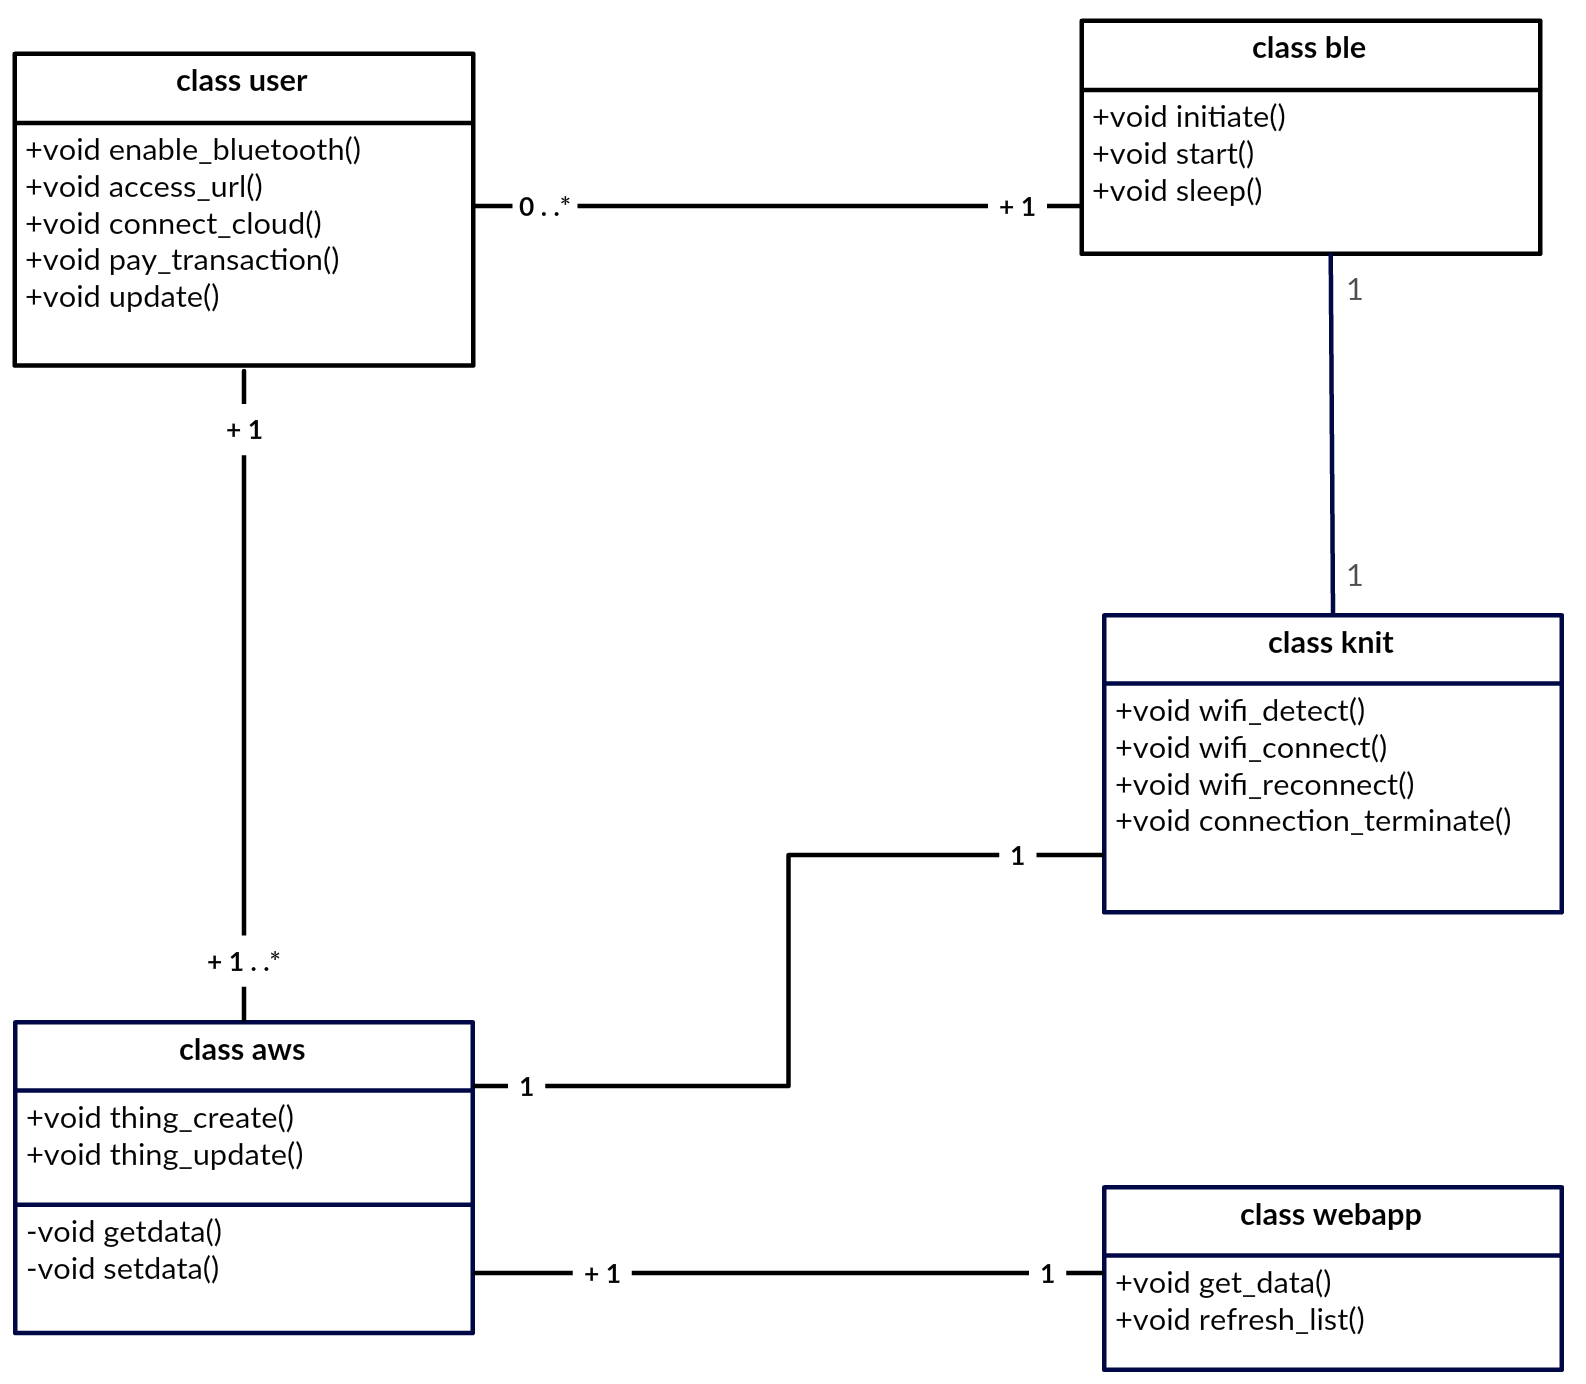
\includegraphics[width=450pt]{class.png}}
	  \caption{Class Diagram}
	  \label{fig:class-dig}
	\end{figure}
\end{center} 
This diagram depicts the various classes present in the program and the respective data types and functions used in them.

\begin{appendices}
\newpage
\section{Summary and Conclusion}
The project requirements are studied in detail and are fulfilled successfully.This project has enhanced our knowledge and skills.It consists of different technologies and ideas used together to develop an innovative and new platform.  

% \chapter{ALGORITHMIC DESIGN}
\chapter{Laboratory assignments on Project Analysis of Algorithmic Design}




\chapter{Laboratory assignments on Project Quality and Reliability Testing of Project Design}

\chapter{Reviewers Comments of Paper Submitted}

\begin{enumerate}
\item Paper Title: Physical Web with Vending Machine

\item Name of the Conference/Journal where paper can be  submitted :
 Physical Web in Smart Cities - Advances in Wireless and Optical Communications (RTUWO), 2015\\
 On physical web models - Control and Communications (SIBCON), 2016 \\
International Siberian Conference Finite state machine based vending machine – International Journal of VLSI design and communication system 2012.\\


\item Paper accepted/rejected : Not applied yet. 
\item Review comments by reviewer : not yet applied 
\item Corrective actions if any :   not yet applied 

\end{enumerate}

\chapter{Plagiarism Report}
Plagiarism report


\end{appendices}


\end{document}
